% Hand-maintained r14 revision.
% Supersedes the TeXFlow-generated r13 snapshot with a Hossain-style main paper.
% Audit detail moved to manuscript/supplement.tex.
\documentclass[11pt,a4paper]{article}

\usepackage{mathptmx}
\usepackage[top=1in,bottom=1in,left=1.1in,right=1.1in]{geometry}
\usepackage{graphicx}
\usepackage[colorlinks=true,linkcolor=black,urlcolor=black,citecolor=black]{hyperref}
\usepackage{url}
\usepackage[numbers,sort&compress]{natbib}
\usepackage{fancyhdr}
\usepackage[font=small,labelfont=bf,justification=centering]{caption}

\linespread{1.0}

% Standard numbered sections (Solar Energy / Elsevier style)
\renewcommand{\thesection}{\arabic{section}}
\renewcommand{\thesubsection}{\arabic{section}.\arabic{subsection}}
% JBSS tables: full grid with heavier rules
\setlength{\arrayrulewidth}{0.8pt}
% JBSS References heading: centered bold
\renewcommand\bibsection{\begin{center}\textbf{References}\end{center}}
% Clean-manuscript running heads (editors add journal chrome)
\pagestyle{fancy}
\fancyhf{}
\fancyhead[L]{\small\textit{Siddiquee and Fahim}}
\fancyhead[R]{\small\textit{Modeling Electrical Losses}}
\fancyfoot[C]{\thepage}
\renewcommand{\headrulewidth}{0pt}

\title{Modeling electrical losses in CsPbI3 solar cells: stacked idealizations and a routine-quality envelope at 18.0\%}
\author{Hussain Touhid Siddiquee\thanks{Department of EEE, Leading University, Sylhet-3112, Bangladesh. E-mail: \url{touhidsiddiqueeraj@gmail.com}, \url{mdabdulmalekfahim@gmail.com}.} \and Md.\ Abdul Malek Fahim}
\date{}

\begin{document}
\maketitle

\begin{quote}\small
Stacked idealisations inflate SCAPS-1D CsPbI3 projections. On one fully worked CsPbI3/CBTS stack, joint optimisation of thickness, doping, defects, gap, and both transport-layer affinities gives a permissive-box ceiling of \textbf{24.95\%}. Sampling a frozen routine-quality prior volume (96-point Latin hypercube over eight factors; ranges and measured anchors in Table~\ref{tab:prior}) gives a median of \textbf{18.0\%} with a 5--95\% prior-predictive envelope of \textbf{15.6--20.0\%}. This is a sensitivity envelope under stated priors, not a confidence interval on real devices. The 2024--2026 experimental records fall above that envelope. The ceiling record comparison is density-of-states conditional: with capped density of states, literature radiative recombination ($C_r=10^{-10}$~cm$^3$/s) lowers the ceiling to 21.86\%, below the 22.02\% certified record; with effective-mass physical density of states, the same radiative term gives 23.46\% ($N_v=4.1\times10^{18}$~cm$^{-3}$) and 23.04\% ($N_v=8.9\times10^{18}$~cm$^{-3}$), above it. Interface sensitivity is regime dependent, bulk defects dominate at routine defect density, and series resistance up to 5~$\Omega$cm$^2$ closes roughly half of the six-point fill-factor gap against measured devices, with the remainder attributed to nonradiative interface recombination (ideality above unity).
\end{quote}

\medskip
\noindent{\small\textbf{Keywords:} CsPbI3; perovskite solar cell; SCAPS-1D; CBTS; reproducibility; device simulation}
\par

\section{Introduction}

All-inorganic CsPbI3 combines improved thermal stability with a bandgap near 1.7~eV, suitable for single-junction and tandem top-cell use~\cite{Dai2026,Qiu2025}. Buried-interface engineering carried laboratory efficiencies past 20\% in 2024~\cite{Shah2024} and to 22\% in 2025--2026: 22.60\% laboratory and 22.02\% certified by moisture-responsive crystallisation~\cite{Dai2026}, 22.05\% by fluorinated interfacial dipoles~\cite{Qiu2025}, with supporting records of 21.71\% with dual-interface and bulk co-passivation at 1.27~V~\cite{Zhang2026} and 21.43\% certified for inverted cells~\cite{Joule2026}. The 22.02\% certified value of Dai et al.\ is the highest certified CsPbI3 value cited here. Each advance came from defect and interface control.

SCAPS-1D is widely used for pre-experimental screening. The ITO/TiO2/CsPbI3/CBTS stack of \citet{Hossain2023} progressed from 17.90\% over 96 transport-layer combinations~\cite{Hossain2022} to 19.06\% after optimisation. Later simulation reports reach 24.17\% on the same stack~\cite{Nazli2025} and 24.24\% on ZnO/PTAA without interface layers~\cite{Oyedele2023}. Three recurring problems accompany this inflation. First, one-variable-at-a-time optimisation hides interactions among thickness, doping, defects, gap, and alignment. Second, interface and defect assumptions are often incompletely reported. Third, scripted SCAPS sweeps can mix unit systems and silently alter defect populations.

A survey of more than 250 SCAPS perovskite architectures attributes much of this inflation to unrealistic inputs, especially the zero radiative-recombination default, unphysical defect floors and mobilities, isolated optimisation, and optical defaults~\cite{Saidarsan2025}. A companion optical-loss framework implements the wavelength-dependent half of that protocol~\cite{Guruprasad2026}. This paper implements the electrical-loss half on one stack: factorial screening, priced radiative, mobility, resistance, contact, affinity, and density-of-states assumptions, and a routine-quality sensitivity envelope.

This work contributes a five-factor guardrailed screen and joint affinity map locating the ceiling at 24.95\%; priced single-assumption corrections; stacked realistic variants; a measured-grade calibration ladder; a 95-run routine-quality envelope with a separate radiative sensitivity subset; interface dose--response in portable lifetime/velocity metrics; and a range-dependent Morris analysis.

\section{Literature: CsPbI3 progress and simulation inflation}

Black-phase CsPbI3 progressed from 10.8\% quantum-dot films through $\gamma$-films and graded-gap devices~\cite{Swarnkar2016,Zhao2018,Bian2018}. Compositional engineering continued this rise~\cite{Xi2019,Becker2019}. The 18.4\% $\beta$-phase result then stood until buried-interface work reached 20.6\%, 20.1\% stabilised~\cite{Wang2019,Shah2024}. The 2025--2026 interface wave is shown in Figure~\ref{fig:timeline}.

\begin{figure}[htbp]
\centering
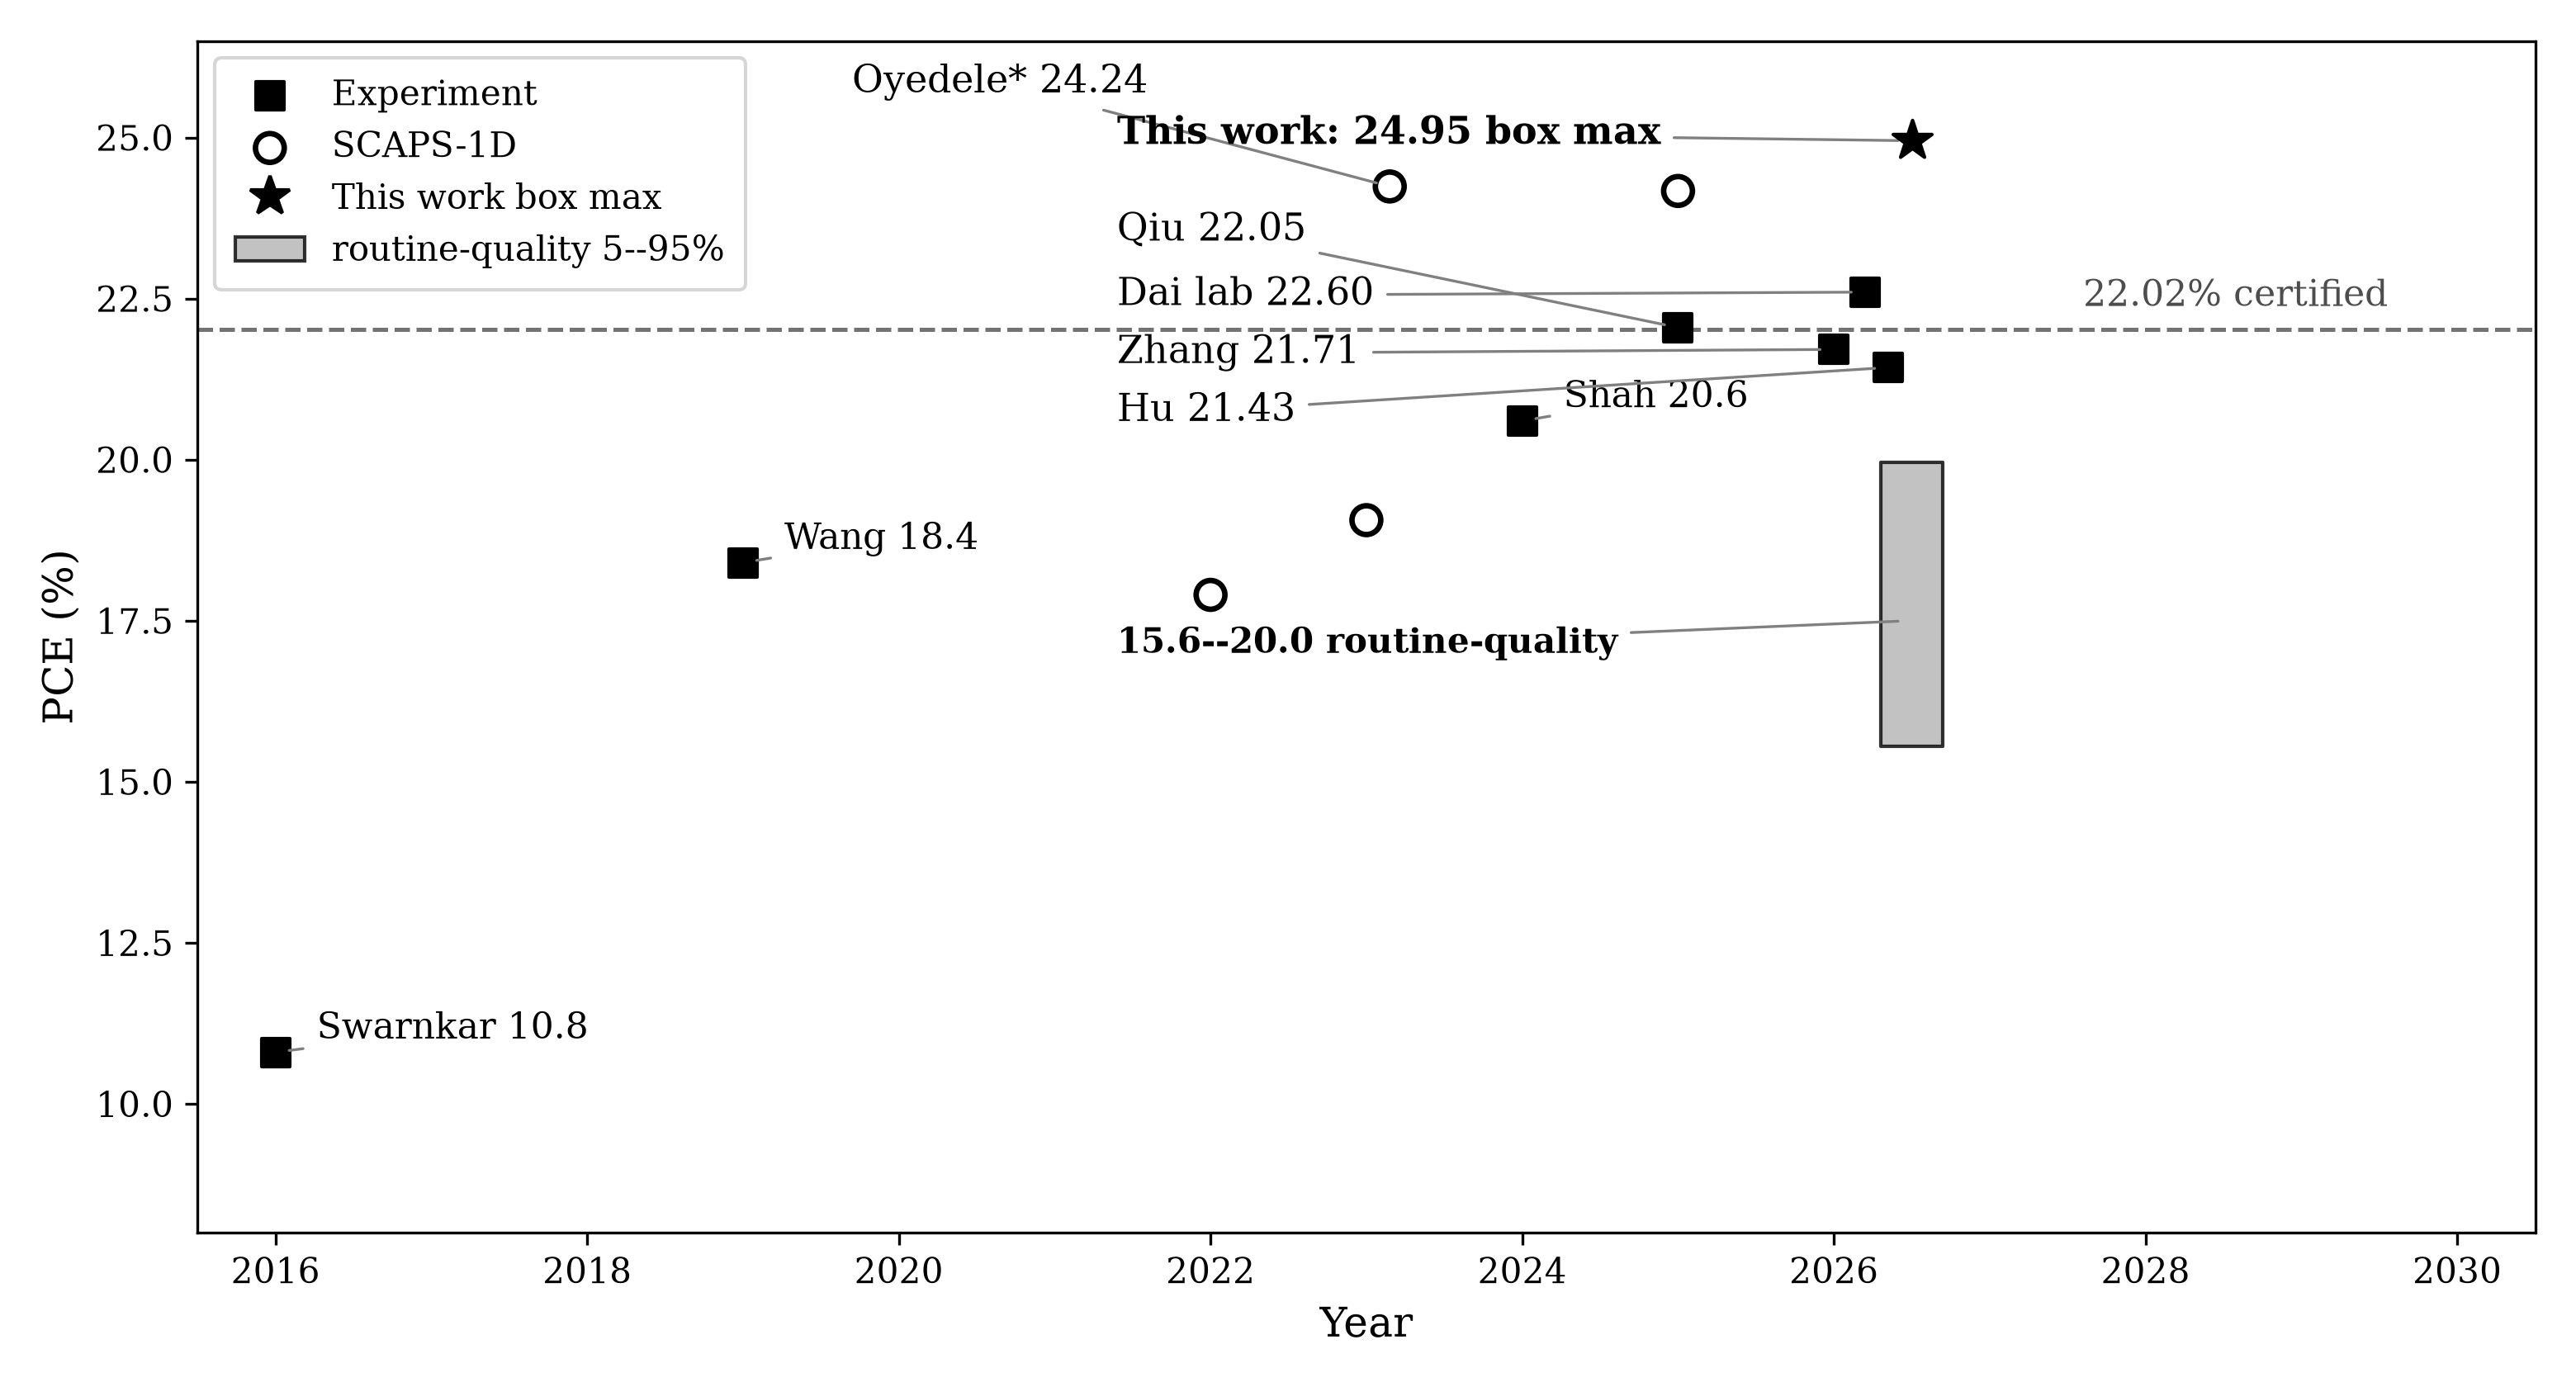
\includegraphics[width=0.95\textwidth]{figs/fig_timeline.png}
\caption{CsPbI3 record race. Open symbols are simulations; the star and band are this work's ceiling and envelope.}
\label{fig:timeline}
\end{figure}

\begin{table}[htbp]
\centering
\caption{Selected CsPbI3 results: experiment versus simulation. Our entry is flagged, not ranked: $^{\star}$permissive-box ceiling; the defended envelope median is 18.0\% with 5--95\% range 15.6--20.0\%. Certified values are marked $^{c}$; other experimental values are laboratory-reported.}
\label{tab:lit}
\small
\begingroup
\setlength{\tabcolsep}{3pt}
\begin{tabular}{|p{0.22\linewidth}|p{0.30\linewidth}|p{0.08\linewidth}|p{0.15\linewidth}|p{0.11\linewidth}|}
\hline\hline
Study & Stack & Type & PCE (\%) & IF \\
\hline
Swarnkar 2016 & TiO2/Spiro/MoOx & Exp. & 10.8~\cite{Swarnkar2016} & -- \\
Wang 2019 & TiO2/Spiro & Exp. & 18.4~\cite{Wang2019} & -- \\
Shah et al. 2024 & TiO2/2D-Cs2PbI2Cl2 & Exp. & 20.6 (20.1 stab.)~\cite{Shah2024} & buried-passivated \\
Qiu 2025 & CsPbI3 + DFAz dipole & Exp. & 22.05~\cite{Qiu2025} & passivated \\
Zhang 2026 & TiO2 dual-interface+bulk & Exp. & 21.71~\cite{Zhang2026} & co-passivated \\
Dai 2026 & TiO2/PTABr/Spiro & Exp. & 22.60 lab / 22.02$^{c}$~\cite{Dai2026} & passivated \\
Hu 2026 (Joule) & inverted HPDA & Exp. & 21.43$^{c}$~\cite{Joule2026} & 2D-stitched \\
Lei 2025 & AP-modified CsPbI3 & Exp. & 22.16~\cite{Lei2025} & passivated \\
Xu 2026 & QD-interface, inverted & Exp. & 22.15~\cite{XuQD2026} & QD-passivated \\
Hossain 2022 & TiO2/CBTS & Sim. & 17.90~\cite{Hossain2022} & on \\
Hossain 2023 & TiO2/CBTS/Ni & Sim. & 19.06~\cite{Hossain2023} & on \\
Nazli 2025 & TiO2/CBTS/Ni & Sim. & 24.17~\cite{Nazli2025} & unclear \\
Oyedele 2023 & ZnO/PTAA & Sim. & 24.24~\cite{Oyedele2023} & OFF \\
This work$^{\star}$ & TiO2/CBTS/Ni & Sim. & 24.95 & on \\
\hline\hline
\end{tabular}
\endgroup
\end{table}

The simulation studies trace a parallel inflation curve. The CBTS programme reached 17.90\% and 19.06\%~\cite{Hossain2022,Hossain2023}, the re-parameterised baseline used here. Later claims report higher values on different stacks or with unclear interface treatment. Because several published parameter tables are incomplete, other groups' cells are compared as reported, not re-placed on our curve.

\section{Numerical simulations}

\subsection{SCAPS-1D model}

SCAPS-1D solves Poisson's equation with electron and hole continuity under drift-diffusion transport~\cite{Burgelman2000,Khattak2019,BurgelmanSCAPS}:
\begin{equation}
-\frac{\partial}{\partial x}\left(\varepsilon(x)\frac{\partial V}{\partial x}\right) = q[p-n+N_D^+-N_A^-+p_t-n_t],
\end{equation}
\begin{equation}
\frac{\partial n}{\partial t}=\frac{1}{q}\frac{\partial J_n}{\partial x}+G_n-R_n,\quad
\frac{\partial p}{\partial t}=-\frac{1}{q}\frac{\partial J_p}{\partial x}+G_p-R_p,
\end{equation}
\begin{equation}
J_n=q\mu_nnE+qD_n\nabla n,\quad
J_p=q\mu_ppE-qD_p\nabla p,
\end{equation}
with Shockley--Read--Hall recombination through the specified bulk and interface defect levels. Optical generation uses the Eg-sqrt model, $\alpha=A\sqrt{h\nu-E_g}$, so gap sweeps move the absorption edge rather than using a frozen spectrum.

\subsection{Device structure and re-parameterised baseline}

Devices were simulated under AM1.5G illumination at 100~mW/cm$^2$ and 300~K unless stated. The starting point reproduces \citet{Hossain2023}: ITO, 30~nm TiO2, CsPbI3, 100~nm CBTS, and Ni. Neutral interface recombination blocks are present at both heterojunctions. The absorber uses the edge-moving absorption model. This is therefore a re-parameterised baseline, not an unmodified copy: interfaces were added and the density-of-states treatment is stated explicitly.

The re-parameterised baseline gives 18.99\% (Voc 1.122~V, Jsc 19.68~mA/cm$^2$, FF 86.00\%), within the published 17.9--19.06\% band. Doping and defect floors remain modelling choices; measured doping is far lower~\cite{PenaCamargo2022}. Using the source paper's printed density of states instead gives 16.76\%, so baseline replication depends materially on that choice.

\begin{table}[tbp]
\centering
\caption{Layer input parameters for the re-parameterised baseline. Screening subsequently moves ETL doping to $9\times10^{17}$~cm$^{-3}$ and explores ETL affinity; the ceiling values are in Table~\ref{tab:champ}.}
\label{tab:in}
\resizebox{\linewidth}{!}{%
\begin{tabular}{|l|l|l|l|l|l|l|l|}
\hline\hline
Layer & $d$ & $E_g$ & $\chi$ & $\varepsilon_r$ & Doping & $N_t$ & $\mu_{n}/\mu_{p}$ \\
\hline
CBTS HTL & 100~nm & 1.9 & 3.6 & 5.4 & $N_A$ 1e18 & 1e15 & 30/30 \\
CsPbI3 & 800~nm & 1.694 & 3.95 & 6.0 & $N_A$ 1e15 & 1e15 & 25/25 \\
TiO2 ETL & 30~nm & 3.2 & 4.0 & 9.0 & $N_D$ 9e16 & 1e15 & 20/20 \\
\hline\hline
\end{tabular}}
\end{table}

\begin{table}[tbp]
\centering
\caption{Interface defect layers at both heterojunctions: neutral single level, $\sigma=10^{-19}$~m$^2$, $E_t=0.6$~eV.}
\label{tab:if}
\begin{tabular}{|l|l|l|}
\hline\hline
Interface & $N$ (cm$^{-2}$) & Sweep range \\
\hline
CBTS/CsPbI3 & 1e10 & $10^8$--$10^{12}$ \\
CsPbI3/TiO2 & 1e10 & $10^8$--$10^{12}$ \\
\hline\hline
\end{tabular}
\end{table}

\subsection{Guardrails and simulation bases}

Guardrails are part of the stated simulation box, not post-hoc filters. The bulk floor is $10^{12}$~cm$^{-3}$ and the interface floor is $10^{10}$~cm$^{-2}$; points below the interface floor are audit points. Energetic screens reject Voc above the radiative bound or fill factor above Green's ideal-diode value.

\begin{table}[tbp]
\centering
\caption{Guardrails and their anchors. ``Assumption'' means a modelling choice without a direct measurement behind it.}
\label{tab:guard}
\small
\begingroup
\setlength{\tabcolsep}{3pt}\begin{tabular}{|p{0.19\linewidth}|p{0.34\linewidth}|p{0.34\linewidth}|}
\hline\hline
Guardrail & Value & Anchor \\
\hline
Bulk defect floor & $N_t=10^{12}$~cm$^{-3}$ & beyond-best-film lifetime guardrail \\
Interface floor & $N_{if}=10^{10}$~cm$^{-2}$ & assumption; demanding passivation regime \\
Capture cross-section & $\sigma=10^{-19}$~m$^2$ & assumption; swept $\times$0.1--$\times$10 \\
Radiative coefficient & $C_r=0$, priced at $10^{-10}$/$10^{-9}$~cm$^3$/s & assumption; literature bracket tested \\
Mobilities & 25/25 absorber, priced & assumption; DFT-grade values tested \\
Parasitics & scripted $R_s$/$R_{sh}$ & computed, not assumed zero \\
Contacts and affinities & stated and priced & surveyed versus adopted values separated \\
Optics & flat 10\% reflection, edge-moving absorption & upper-envelope blue response; uncertainty carried \\
Screens & model-derived Voc and ideal-FF bounds & automated receipt gates; see Supplement \\
\hline\hline
\end{tabular}
\endgroup
\end{table}

Five bases recur in the paper and are defined once in Table~\ref{tab:bases}.

\begin{table}[tbp]
\centering
\caption{Simulation bases. Absorber affinity follows $\chi=3.95+0.5(E_g-1.694)$ unless a transport-layer affinity adoption is stated.}
\label{tab:bases}
\small
\begingroup
\setlength{\tabcolsep}{3pt}
\begin{tabular}{|p{0.20\linewidth}|p{0.30\linewidth}|p{0.38\linewidth}|}
\hline\hline
Base & Definition & Carries \\
\hline
Surveyed & Hossain parameters: $\chi_{\mathrm{CBTS}}=3.6$, $\chi_{\mathrm{TiO2}}=4.0$, $E_g=1.694$, 0.8~$\mu$m & baseline 18.99\% \\
Prior adopted & surveyed plus $N_D=9\times10^{17}$, $E_g=1.65$, $\chi_{\mathrm{TiO2}}=3.8$ & dose/audit anchor 23.84\% \\
Ceiling & adopted plus $\chi_{\mathrm{CBTS}}=3.9$, $\chi_{\mathrm{TiO2}}=3.7$, 2.2~$\mu$m, $N_A=3\times10^{16}$, $N_t=10^{12}$ & 24.95\% ceiling \\
Routine & surveyed transport affinities ($\chi_{\mathrm{CBTS}}=3.6$, $\chi_{\mathrm{TiO2}}=4.0$), $E_g=1.65$, 1.0~$\mu$m, $N_A=3\times10^{16}$, $N_D=9\times10^{17}$, $N_t=10^{15}$ & reference 20.82\% \\
Calibration & surveyed transport affinities, $E_g=1.70$, ITO 4.2~eV (dedicated def variant; stacked variants use ITO 4.4~eV), $R_s=1$ & ladder 19.33--20.66\% \\
\hline\hline
\end{tabular}
\endgroup
\end{table}

\section{Results and discussion}

\subsection{Grid screen and permissive-box ceiling}

Round~A screened thickness, acceptor density, bulk defects, ETL doping, and gap in one 96-run batch. Round~B refined thickness, gap, and doping in 36 runs. The surveyed-affinity best reached 23.50\%. Joint mapping of both transport-layer affinities then located the permissive-box ceiling at $\chi_{\mathrm{CBTS}}=3.9$ and $\chi_{\mathrm{TiO2}}=3.7$~eV.

\begin{table}[tbp]
\centering
\caption{Ceiling-point parameters and result. This is the highest evaluated guardrail-satisfying configuration on the named geometries, not a proven global optimum.}
\label{tab:champ}
\resizebox{\linewidth}{!}{
\begin{tabular}{|l|l|l|l|l|l|}
\hline\hline
Layer & $d$ & $E_g$ (eV) & $\chi$ (eV) & Doping (cm$^{-3}$) & $N_t$ (cm$^{-3}$) \\
\hline
CBTS HTL & 100~nm & 1.9 & 3.9 & NA 1e18 & 1e15 \\
CsPbI3 absorber & 2.2~$\mu$m & 1.65 & 3.928 & NA 3e16 & 1e12 \\
TiO2 ETL & 30~nm & 3.2 & 3.7 & ND 9e17 & 1e15 \\
Interfaces (both) & -- & -- & -- & -- & 1e10 cm$^{-2}$ \\
Result & \multicolumn{5}{l|}{Voc 1.321~V, Jsc 21.20~mA/cm$^2$, FF 89.11\%, PCE 24.95\%} \\
\hline\hline
\end{tabular}}
\end{table}

Here 3.928~eV is the absorber affinity implied by the gap--affinity link at 1.65~eV, not an ETL affinity. The ETL affinity at the ceiling is 3.7~eV and the HTL affinity is 3.9~eV.

\begin{table}[tbp]
\centering
\caption{Joint affinity map at guardrailed interfaces, PCE in percent. The peak turns over past $\chi_{\mathrm{CBTS}}\approx3.95$~eV.}
\label{tab:chia}
\begin{tabular}{|l|l|l|l|l|}
\hline\hline
$\chi_{\mathrm{CBTS}}$ $\backslash$ $\chi_{\mathrm{TiO2}}$ & 3.7 & 3.8 & 3.9 & 4.0 \\
\hline
3.50 & 22.10 & 22.10 & 22.10 & 22.07 \\
3.60 & 23.83 & 23.82 & 23.80 & 23.50 \\
3.70 & 24.67 & 24.64 & 24.53 & 23.77 \\
3.80 & 24.89 & 24.86 & 24.67 & 23.81 \\
3.90 & \textbf{24.95} & 24.91 & 24.74 & 23.81 \\
3.95 & 24.94 & 24.90 & -- & -- \\
4.00 & 24.81 & 24.79 & -- & -- \\
4.10 & 23.25 & 23.25 & -- & -- \\
\hline\hline
\end{tabular}
\end{table}

The ceiling sits at aggressive affinities outside surveyed values and at beyond-best-film defect density. It is therefore an upper anchor for the stated box, not a forecast. The JV curves are shown in Figure~\ref{fig:jvboth}, and the thickness--defect interaction is shown in Figure~\ref{fig:contour}.

\begin{figure}[tbp]
\centering
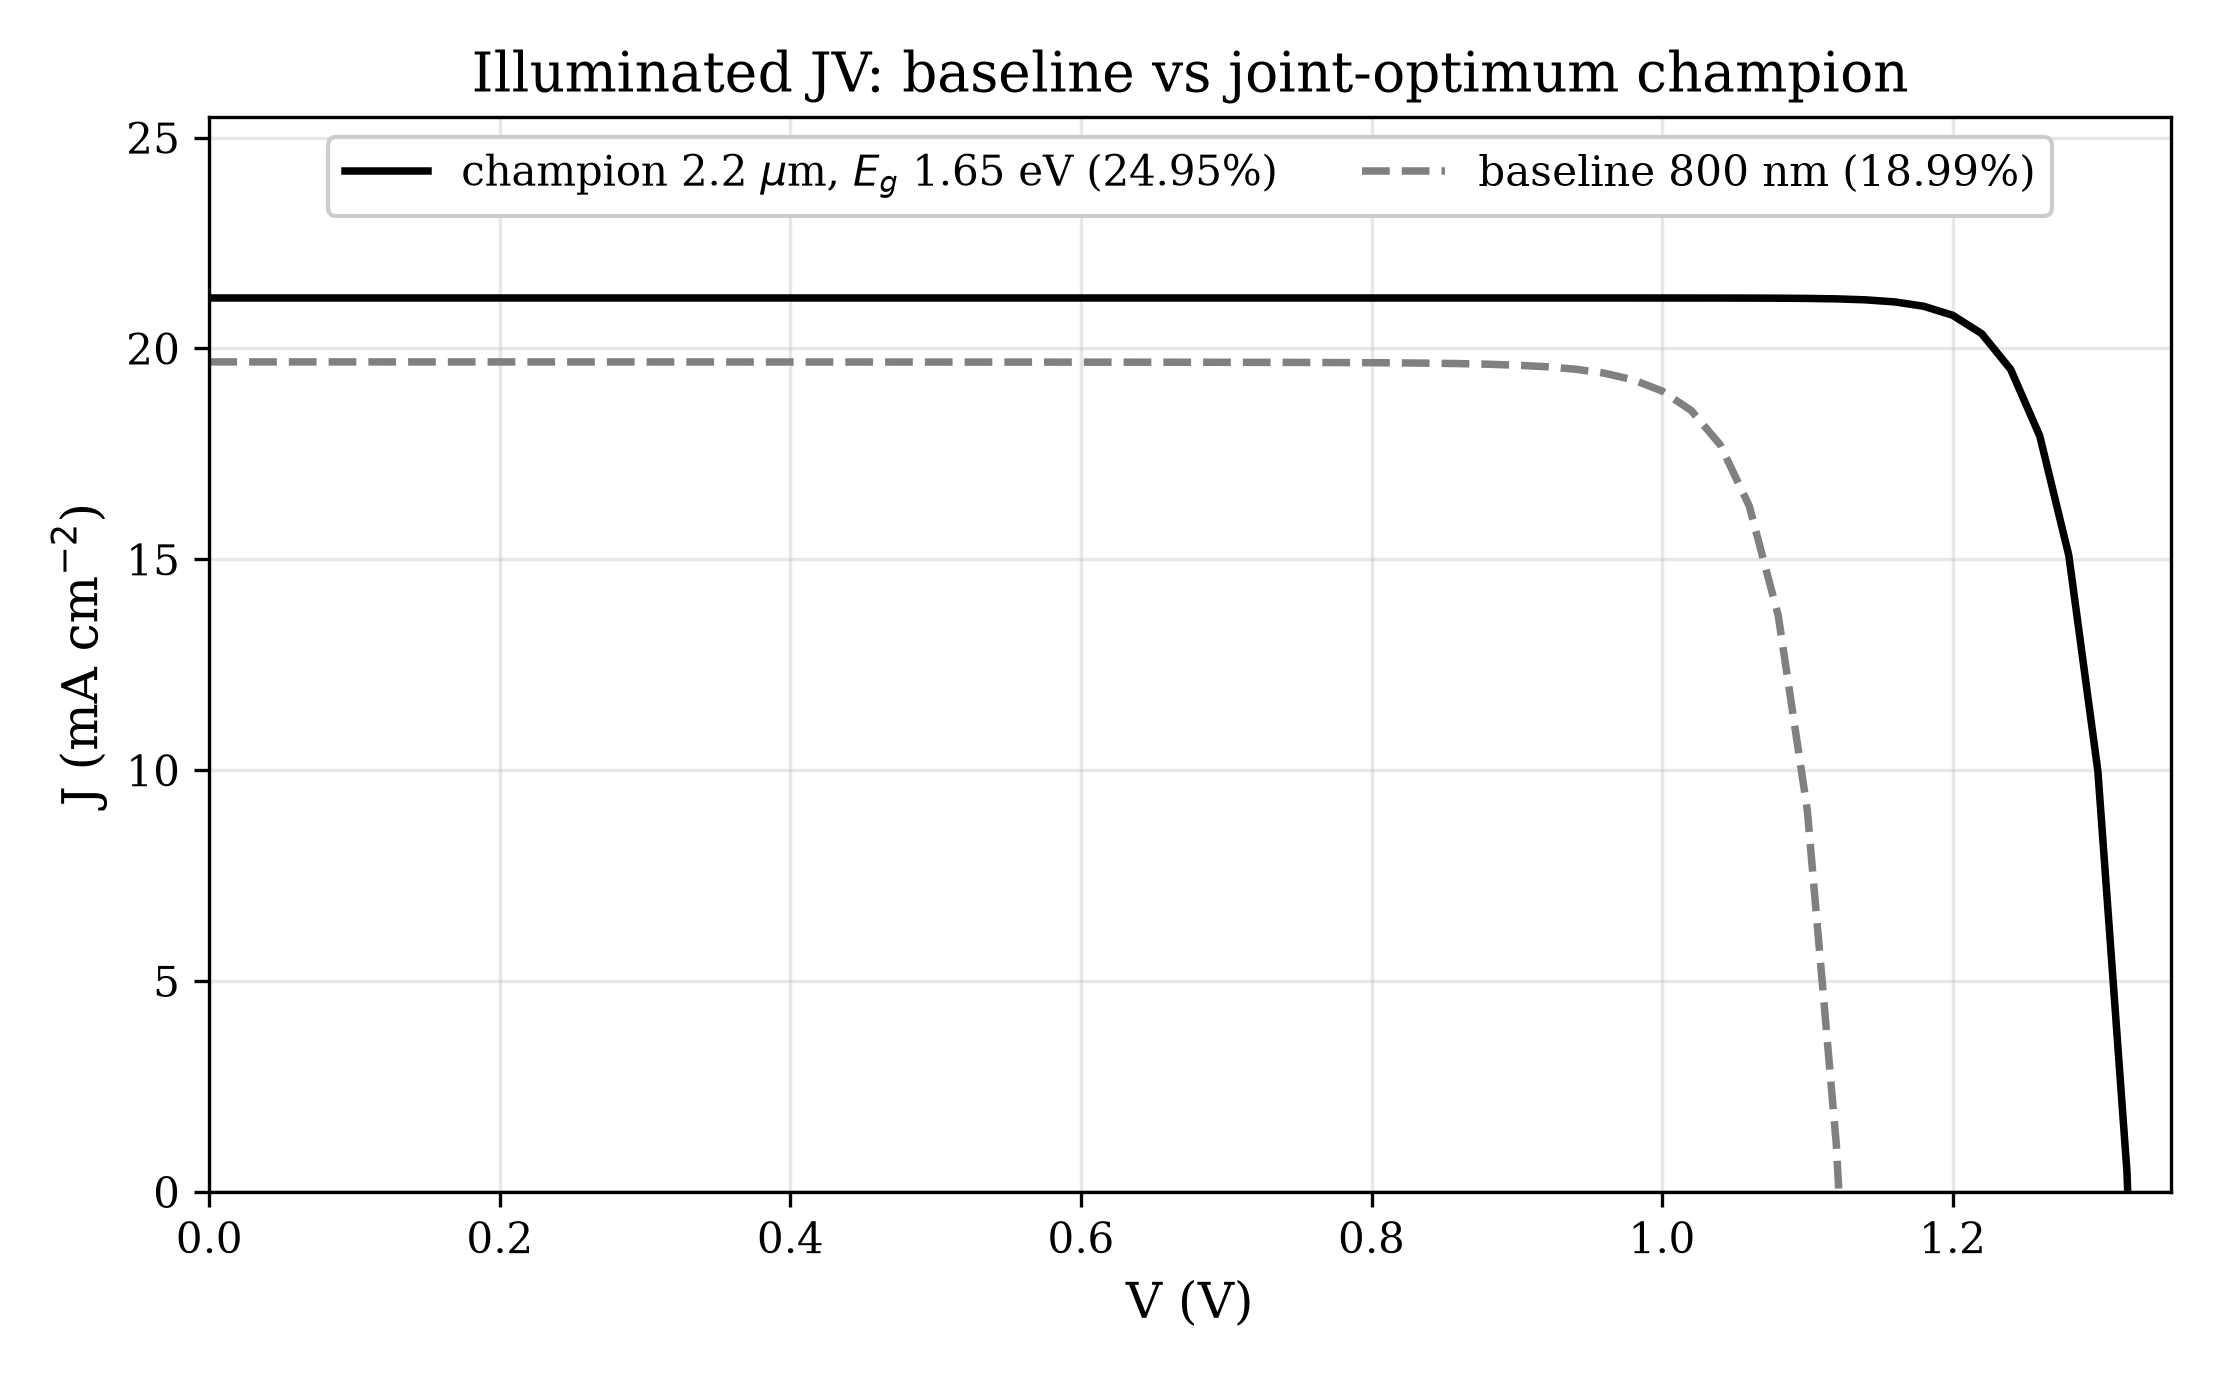
\includegraphics[width=0.85\textwidth]{figs/fig_JVboth.png}
\caption{Illuminated current--voltage curves: re-parameterised baseline versus permissive-box ceiling.}
\label{fig:jvboth}
\end{figure}

\begin{figure}[tbp]
\centering
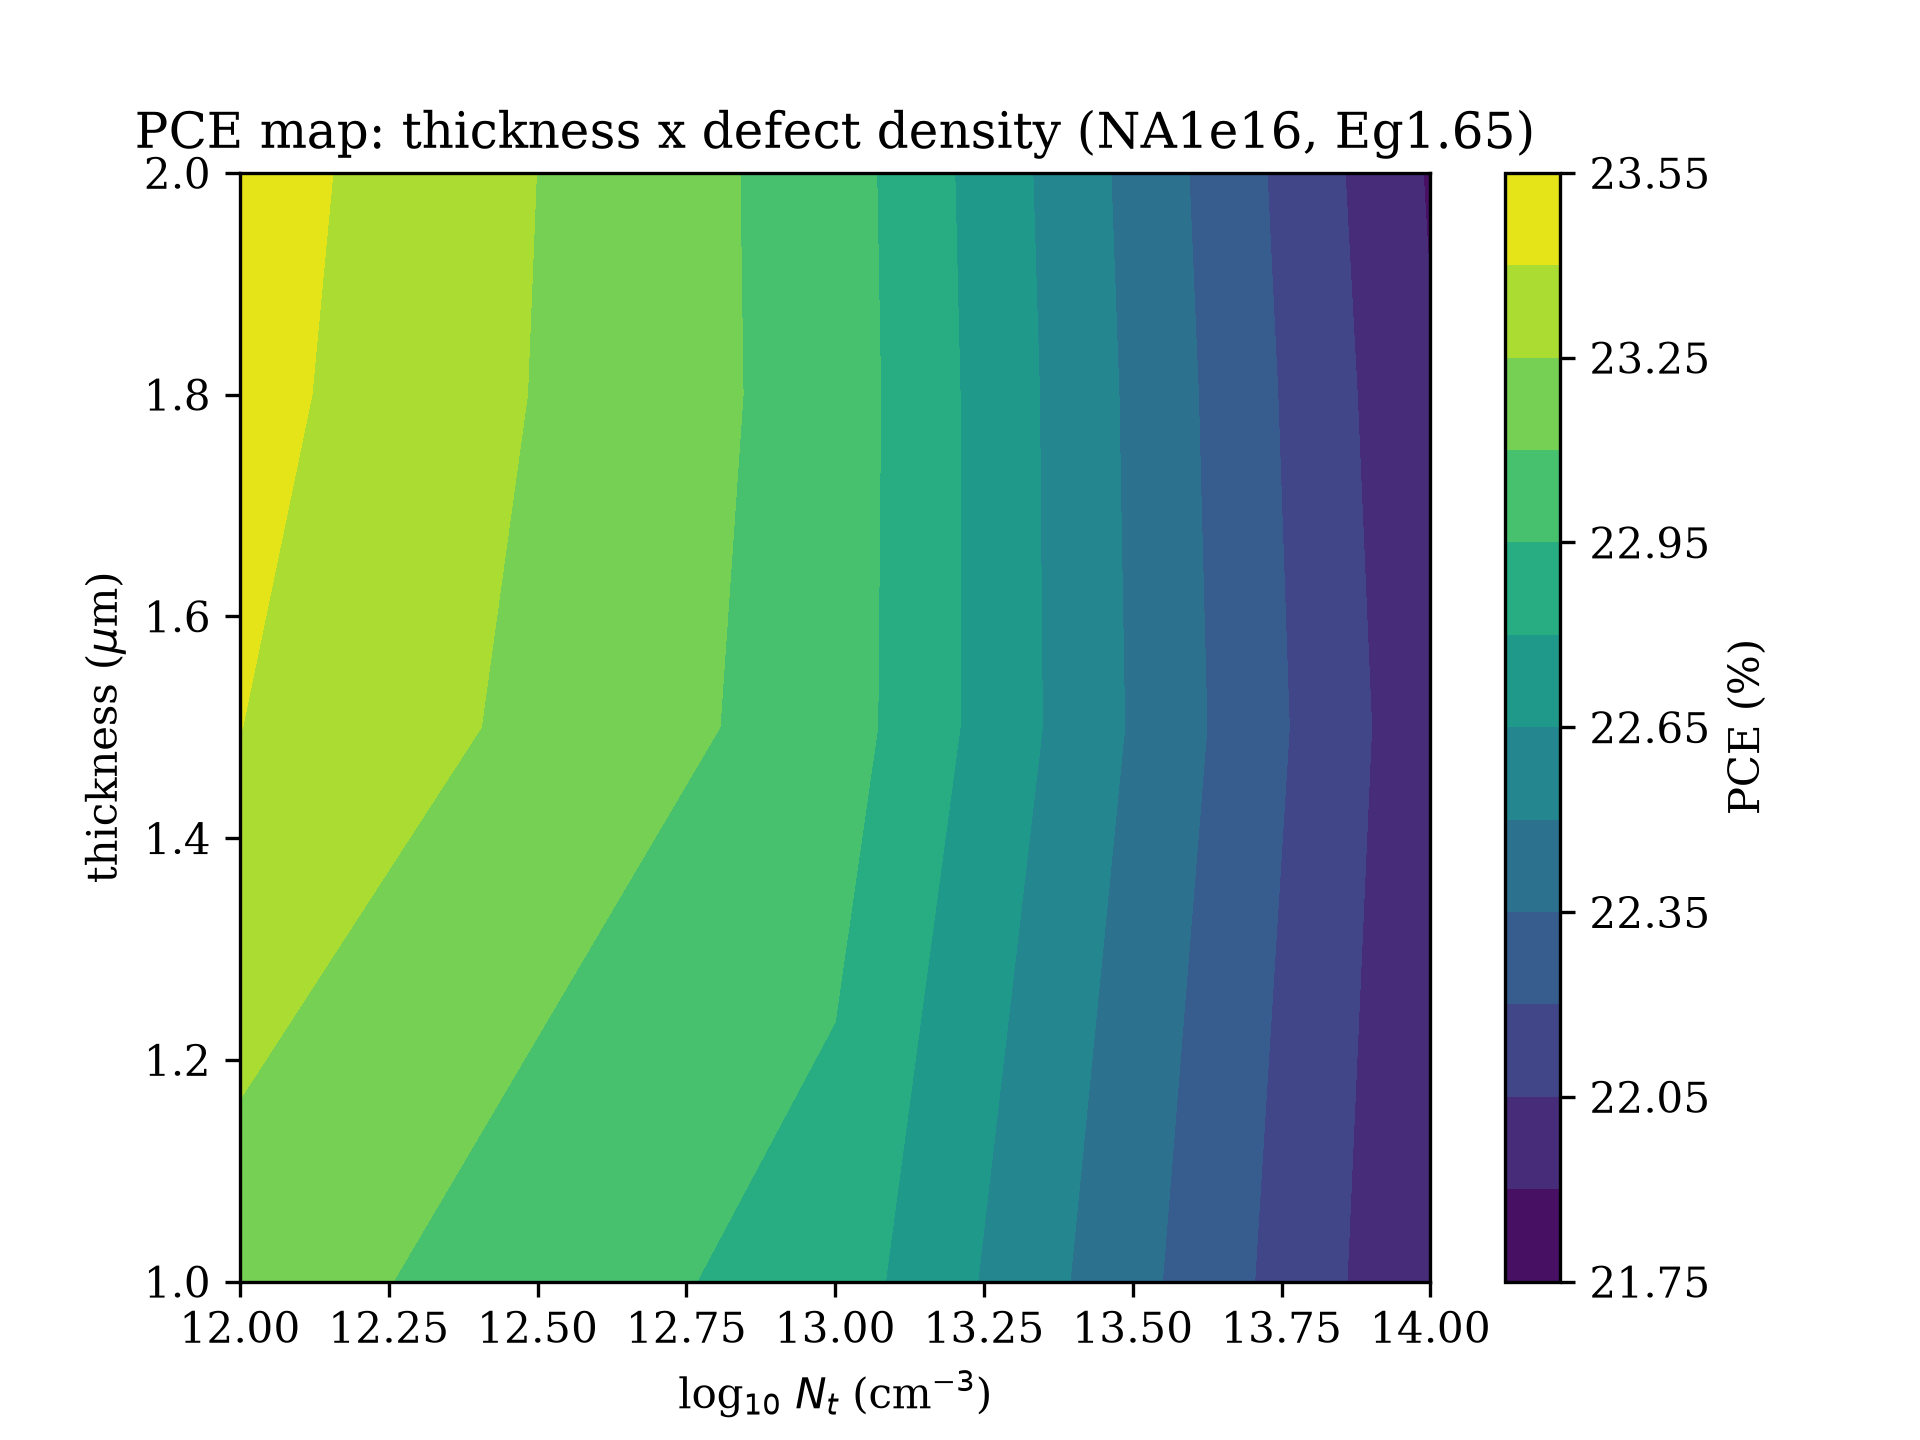
\includegraphics[width=0.8\textwidth]{figs/fig_contour.png}
\caption{Efficiency over absorber thickness and bulk defect density at surveyed transport affinities ($\chi_{\mathrm{CBTS}}=3.6$, $\chi_{\mathrm{TiO2}}=4.0$). The thickness optimum shifts with defect level.}
\label{fig:contour}
\end{figure}

\subsection{Band alignment}

Figure~\ref{fig:align} shows the ceiling alignment from input parameters. The absorber conduction edge lies below the TiO2 edge, while the absorber valence edge lies above the CBTS edge. Efficiency nevertheless peaks there.

\begin{figure}[tbp]
\centering
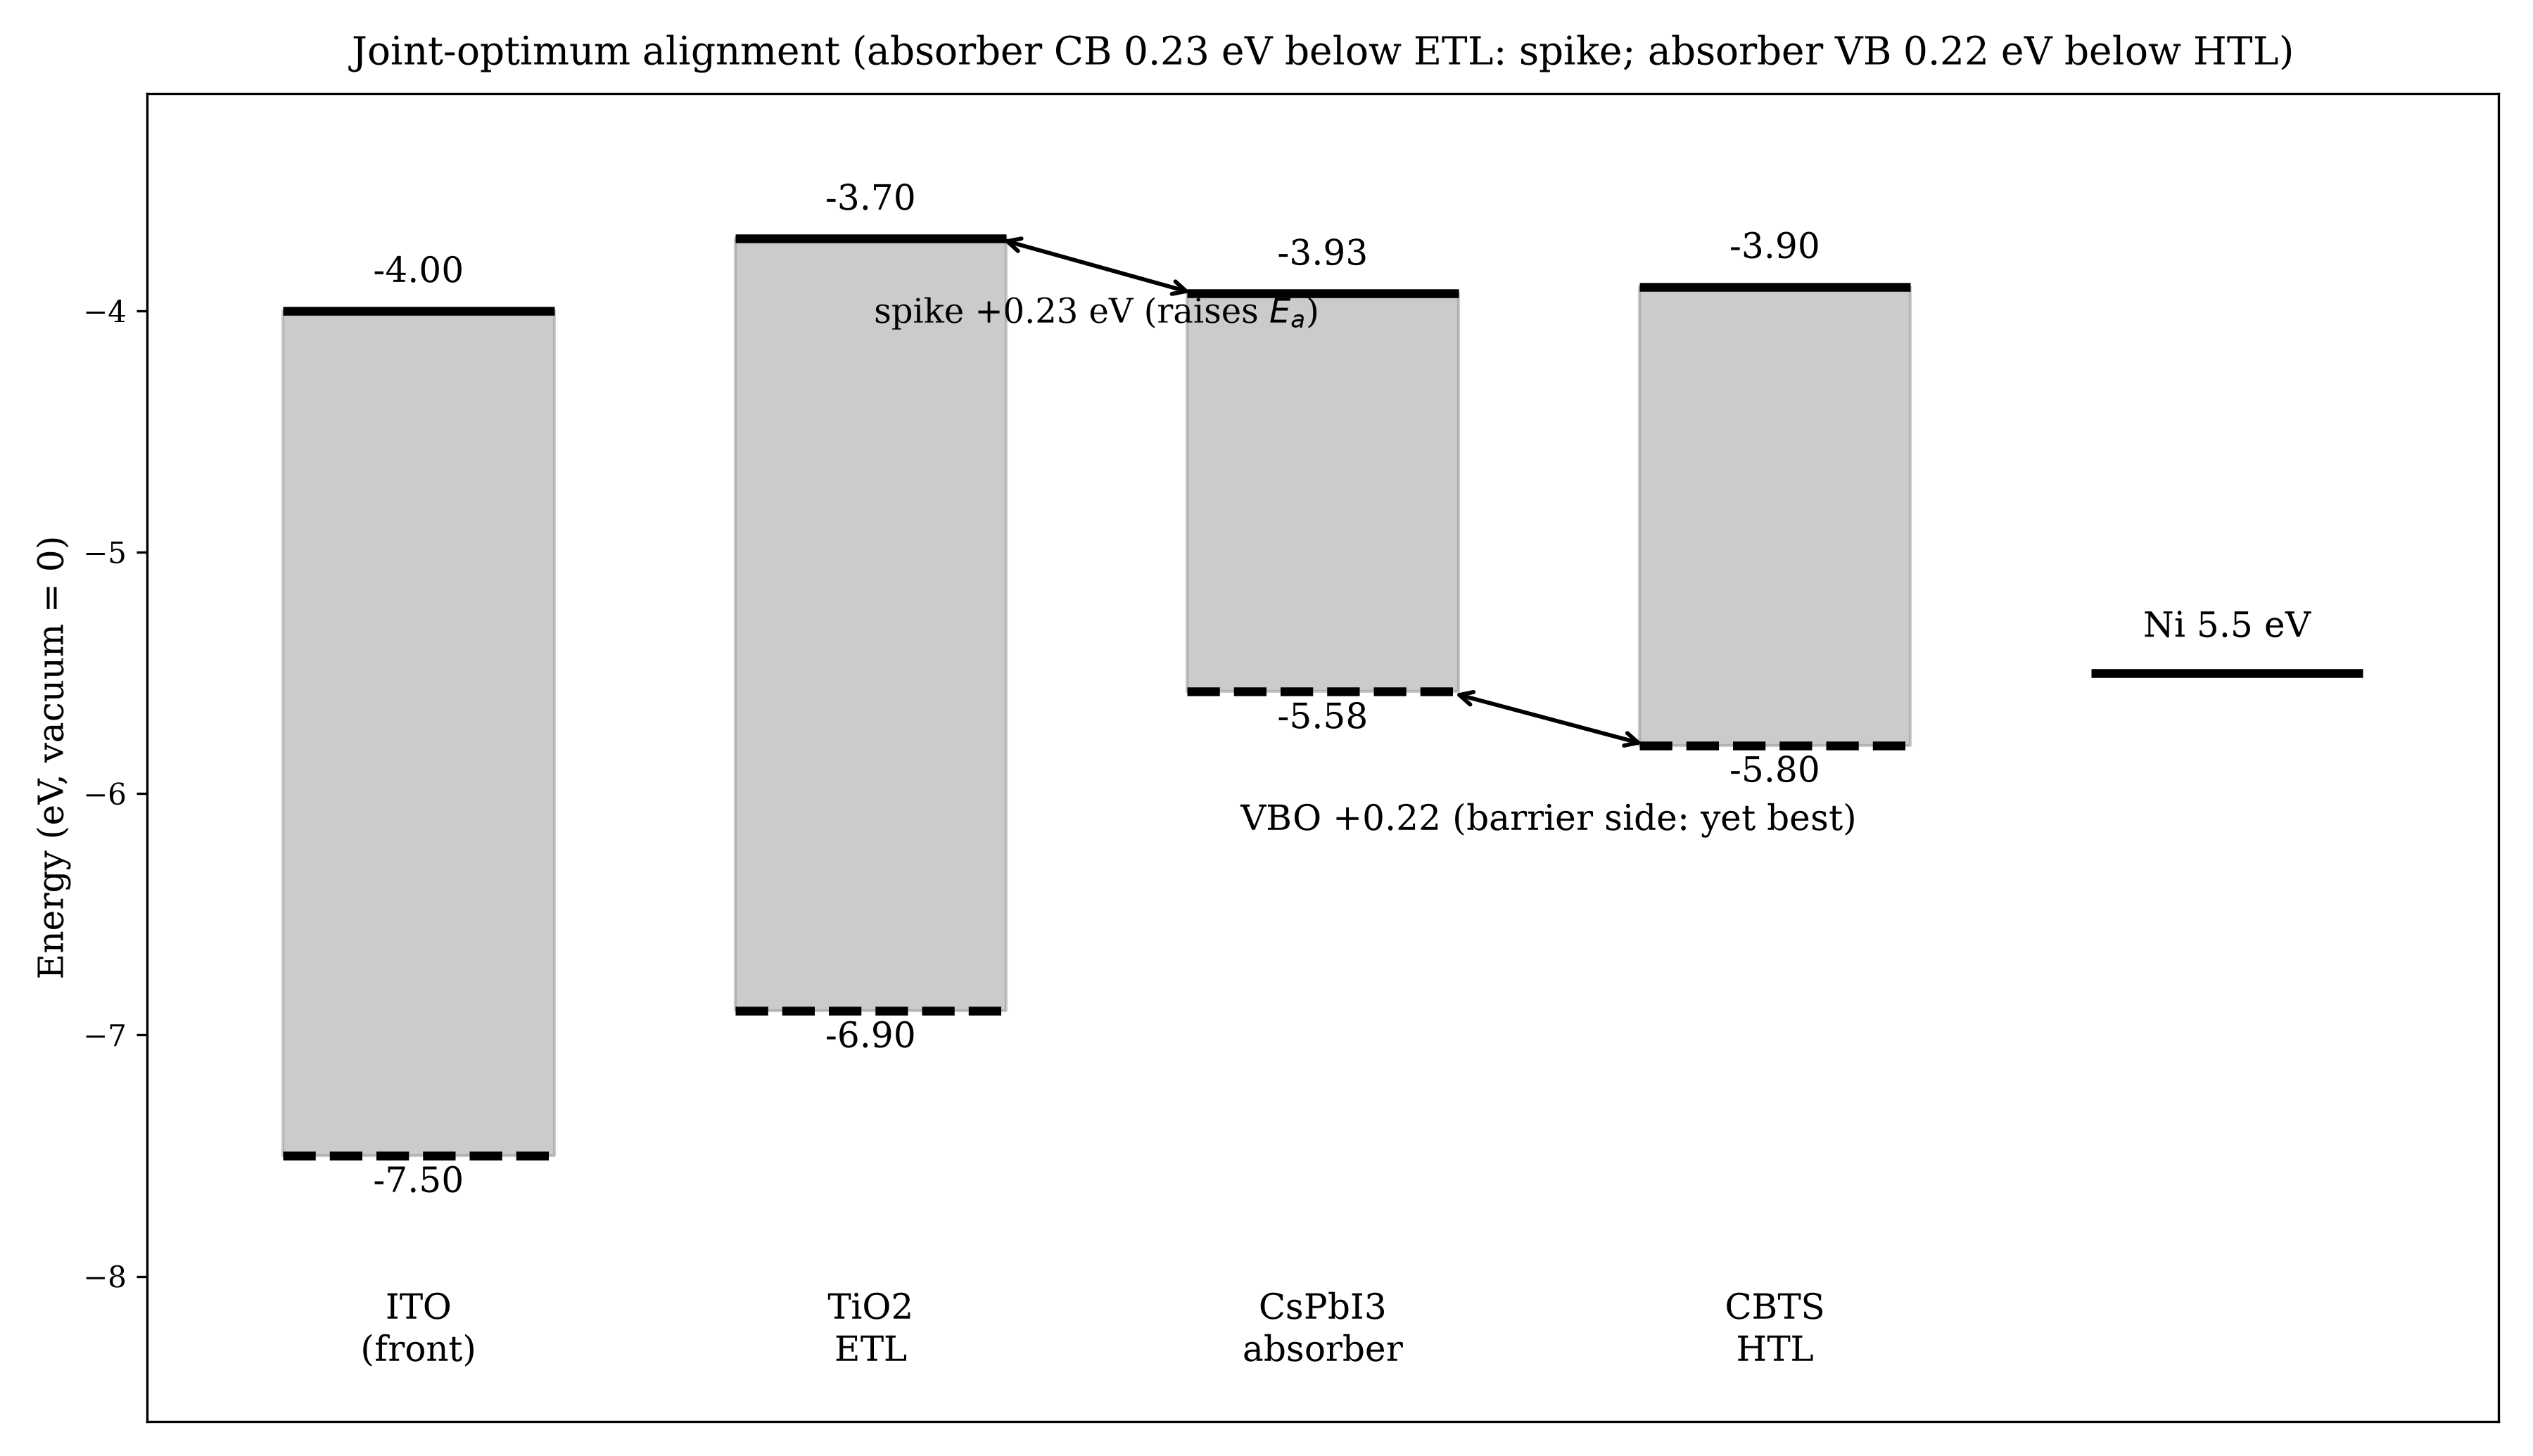
\includegraphics[width=0.8\textwidth]{figs/fig_align.png}
\caption{Equilibrium band alignment of the ceiling stack from input parameters, energies versus vacuum.}
\label{fig:align}
\end{figure}

Two readings can coexist. The interface activation-energy trend supports a recombination reading. The sharp efficiency fall at $\chi_{\mathrm{CBTS}}=4.0$--4.1~eV is also consistent with a growing extraction barrier. The Ni work-function test constrains the contact regime, not the HTL/absorber valence offset, so it does not eliminate the barrier reading. Physical-plausibility flag: the ceiling sits at a 0.23~eV electron spike (absorber conduction edge $-3.928$~eV versus TiO2 $-3.70$~eV) and a 0.22~eV hole barrier (absorber valence $-5.578$~eV versus CBTS $-5.80$~eV) with a Ni contact, both outside surveyed affinity values and with contact cliffs that are partly SCAPS boundary behaviour. The 24.95\% value is therefore retained strictly as a permissive-box upper anchor; the defended number remains the 20.82\% routine-defect result.

\subsection{Device characterisation}

The QE edge moves from 731 to 750~nm between baseline and ceiling cells, supporting the Jsc gain in Figure~\ref{fig:qe}. Because the flat blue plateau assumes no dispersive parasitic absorption, it is an upper envelope rather than a prediction.

\begin{figure}[htbp]
\centering
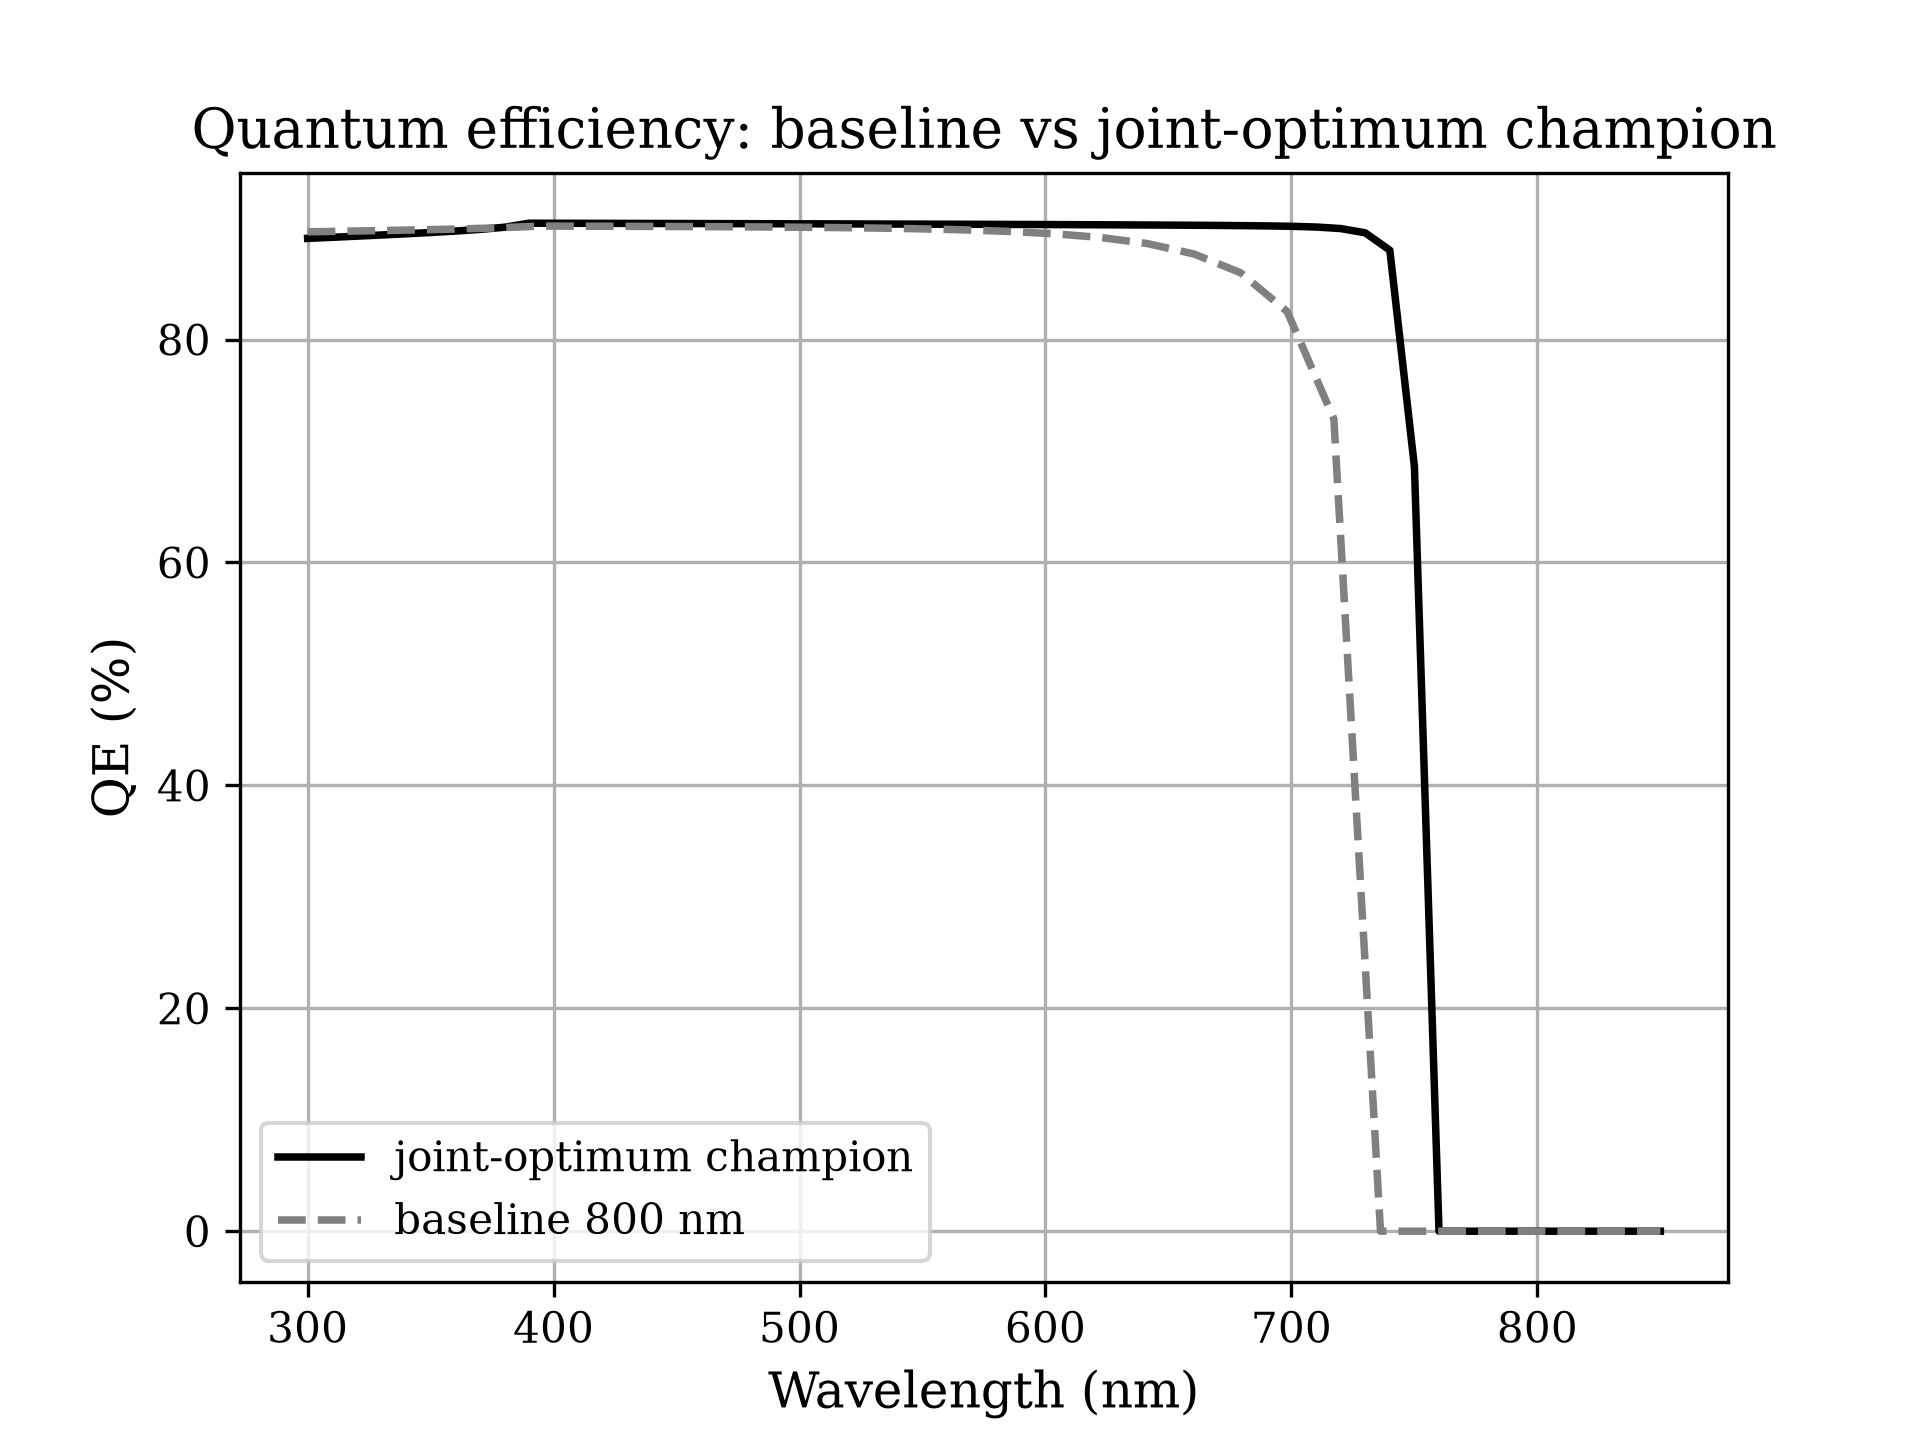
\includegraphics[width=0.8\textwidth]{figs/fig_QE.png}
\caption{Quantum efficiency of baseline versus ceiling cell; the edge shifts 731 to 750~nm.}
\label{fig:qe}
\end{figure}

The computed QE integral is 22.39~mA/cm$^2$ against the converged IV value of 21.20~mA/cm$^2$. For the stated optical stack, independently recomputed ideal step absorption gives 24.4~mA/cm$^2$ at 1.65~eV (23.4 at 1.70~eV, 19.8 at 1.80~eV; receipts \texttt{outputs/s18\_analytic.json}); after the stated 10\% front reflection the 1.65~eV ceiling is 21.96~mA/cm$^2$, below the QE integral. The IV value is therefore retained as the headlined current, with $\pm1.2$~mA/cm$^2$ carried as an absolute-scale systematic. Spectrum-file substitution was blocked by the script interface, so independent spectrum discrimination was not achieved; a manual SCAPS GUI run with the spectrum file selected remains the proposed resolution (Supplement S4 records the blocked test).

Temperature dependence follows the established trend in Figure~\ref{fig:t}: efficiency falls from 25.88\% at 275~K to 18.13\% at 475~K, while Jsc remains near 21.20~mA/cm$^2$. The high-temperature end is a solver stress test because it omits gap narrowing and phase-stability effects.

\begin{figure}[tbp]
\centering
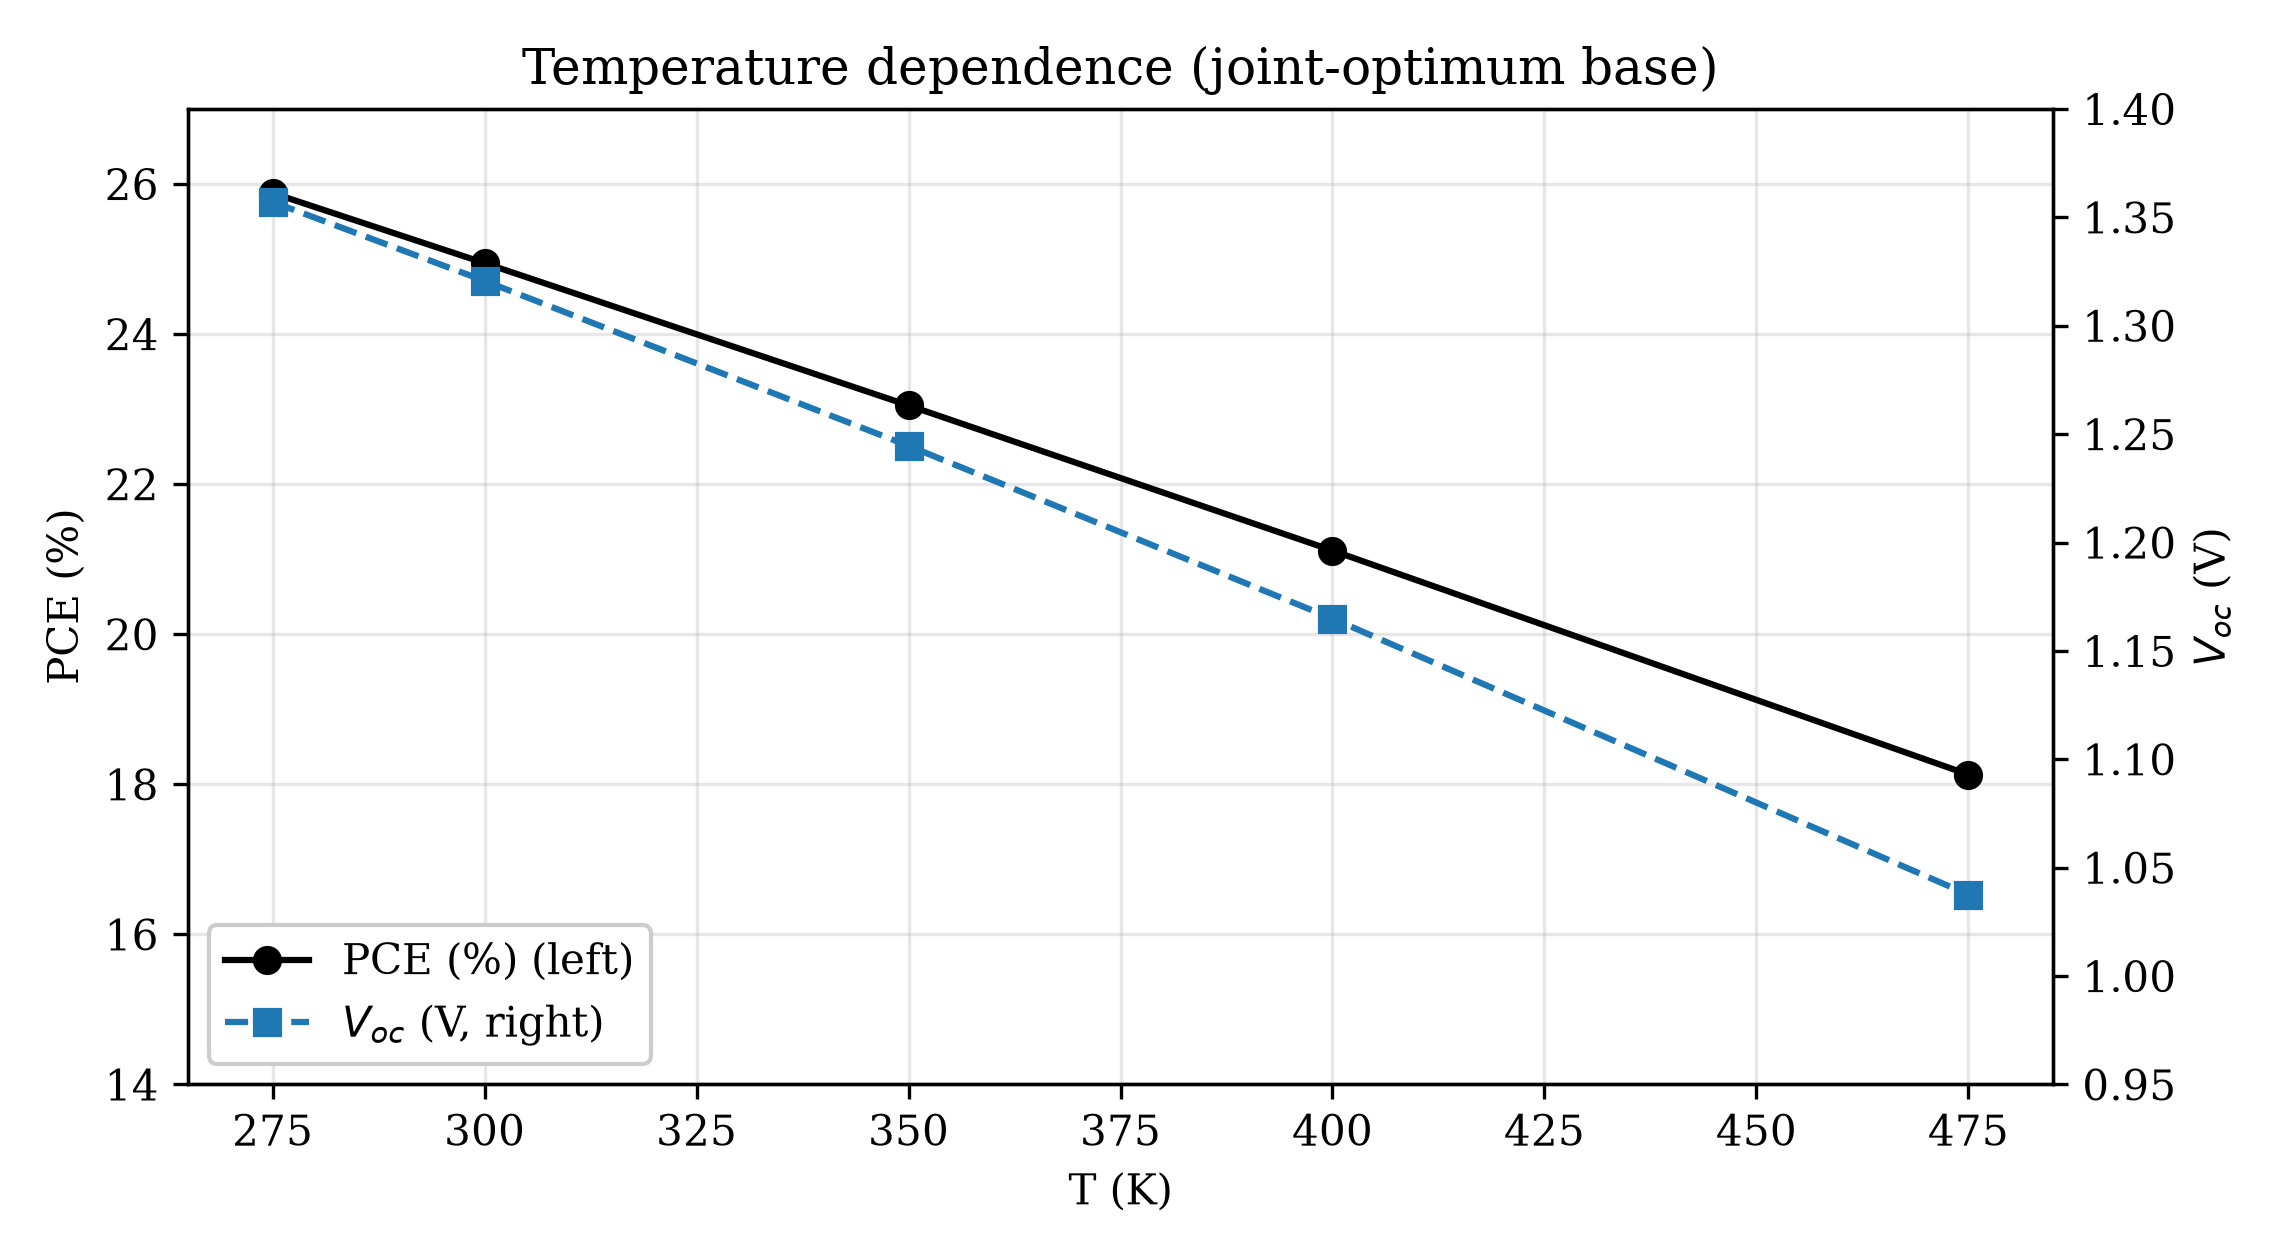
\includegraphics[width=0.8\textwidth]{figs/fig_T.png}
\caption{Efficiency and open-circuit voltage versus temperature at the ceiling base. The 475~K end is a solver stress test.}
\label{fig:t}
\end{figure}

\subsection{Priced radiative, mobility, and parasitic assumptions}

Scripted radiative runs show that the zero-radiative default matters most at the clean corner. At the ceiling it costs 3.09 points at $C_r=10^{-10}$ and 5.12 points at $10^{-9}$~cm$^3$/s. At routine defects the same values cost only 0.14 and 1.02 points. Mobility changes are negligible at the ceiling and 0.32 points at routine defects for DFT-grade 10/5 mobility~\cite{Motta2015}.

\begin{table}[tbp]
\centering
\caption{Pricing the zero-radiative ($C_r=0$) and mobility assumptions against the zero-radiative anchor of each base. $C_r$ denotes the radiative recombination coefficient throughout.}
\label{tab:krad}
\begin{tabular}{|l|l|l|l|l|}
\hline\hline
Run & Voc (V) & Jsc (mA/cm$^2$) & PCE (\%) & $\Delta$ (pts) \\
\hline
Joint optimum ($C_r=0$) & 1.321 & 21.20 & 24.95 & -- \\
$+C_r=10^{-10}$~cm$^3$/s & 1.163 & 21.08 & 21.86 & $-3.09$ \\
$+C_r=10^{-9}$~cm$^3$/s & 1.113 & 20.43 & 19.83 & $-5.12$ \\
$\mu_n$/$\mu_p$ 10/5 & 1.321 & 21.20 & 24.94 & $-0.00$ \\
$\mu_n$/$\mu_p$ 5/2 & 1.321 & 21.20 & 24.94 & $-0.01$ \\
Routine defects ($C_r=0$) & 1.147 & 20.77 & 20.82 & -- \\
$+C_r=10^{-10}$~cm$^3$/s & 1.141 & 20.73 & 20.68 & $-0.14$ \\
$+C_r=10^{-9}$~cm$^3$/s & 1.115 & 20.45 & 19.80 & $-1.02$ \\
$\mu_n$/$\mu_p$ 10/5 & 1.148 & 20.60 & 20.50 & $-0.32$ \\
\hline\hline
\end{tabular}
\end{table}

Scripted parasitics give 24.73\%, 24.52\%, and 24.09\% at $R_s=0.5$, 1, and 2~$\Omega$cm$^2$ on the ceiling base, extending to 23.66\%, 23.23\%, and 22.80\% at $R_s=3$, 4, and 5~$\Omega$cm$^2$ (Table~\ref{tab:rs}). At routine defects, $R_s=1$ lowers 20.82\% to 20.42\%, reaching 19.62\%, 19.22\%, and 18.83\% at $R_s=3$, 4, and 5. Fill factor falls from 89.11\% to 81.45\% on the ceiling base and from 87.42\% to 78.99\% at routine defects across $R_s=0$--5, so resistance alone closes roughly half of the six-point gap to measured fill factors near 83\%; the remainder is attributed to nonradiative interface recombination (ideality above unity), for which illumination-dependent separation data are unavailable.

\begin{table}[tbp]
\centering
\caption{Scripted series-resistance sweep on the ceiling base (2.2~$\mu$m, $N_t=10^{12}$) and the routine base (1.0~$\mu$m, $N_t=10^{15}$), surveyed affinities for the routine column. Receipts in \texttt{outputs/s36\_rs.json} with $R_s=0.5$--2 anchors in \texttt{outputs/s1\_dose.json}.}
\label{tab:rs}
\begin{tabular}{|l|l|l|l|l|}
\hline\hline
$R_s$ ($\Omega$cm$^2$) & Ceiling PCE (\%) & Ceiling FF (\%) & Routine PCE (\%) & Routine FF (\%) \\
\hline
0 & 24.95 & 89.11 & 20.82 & 87.42 \\
1 & 24.52 & 87.57 & 20.42 & 85.70 \\
2 & 24.09 & 86.03 & 20.02 & 84.00 \\
3 & 23.66 & 84.50 & 19.62 & 82.32 \\
4 & 23.23 & 82.97 & 19.22 & 80.65 \\
5 & 22.80 & 81.45 & 18.83 & 78.99 \\
\hline\hline
\end{tabular}
\end{table}

\subsection{Density-of-states conditionality}

The density-of-states assumption controls the record comparison and is therefore stated prominently.

\begin{table}[tbp]
\centering
\caption{Record comparison under two density-of-states branches. Neither branch alone is presented as the unconditional physical result. The two physical-DOS values differ only in the hole density of states: $N_v=4.1\times10^{18}$~cm$^{-3}$ ($m_h^*=0.3$) versus $N_v=8.9\times10^{18}$~cm$^{-3}$ ($m_h^*=0.5$); $N_c$ is unchanged. No-$C_r$ rows fail the model-derived radiative screen and are excluded from ranking.}
\label{tab:dos}
\small
\begingroup
\setlength{\tabcolsep}{3pt}
\begin{tabular}{|p{0.22\linewidth}|p{0.30\linewidth}|p{0.12\linewidth}|p{0.12\linewidth}|p{0.13\linewidth}|}
\hline\hline
Branch & Ceiling treatment & PCE (\%) & Voc (V) & Against 22.02\% \\
\hline
Capped DOS, $C_r=10^{-10}$ & 24.95 to 21.86 & 21.86 & 1.163 & below record \\
Physical DOS ($m_h^*=0.3$), $C_r=10^{-10}$ & J\_dos03\_cr10 & 23.46 & 1.241 & above record \\
Physical DOS ($m_h^*=0.5$), $C_r=10^{-10}$ & J\_dos05\_cr10 & 23.04 & 1.221 & above record \\
Physical DOS ($m_h^*=0.3$), no $C_r$ & J\_dos03 & 26.50 & 1.390 & excluded \\
Physical DOS ($m_h^*=0.5$), no $C_r$ & J\_dos05 & 26.11 & 1.373 & excluded \\
\hline\hline
\end{tabular}
\endgroup
\end{table}

With capped density of states, literature radiative recombination lowers the ceiling to 21.86\% (Voc 1.163~V), below the certified record. With effective-mass physical density of states, the same radiative term gives 23.46\% at Voc 1.241~V ($N_v=4.1\times10^{18}$~cm$^{-3}$) and 23.04\% at Voc 1.221~V ($N_v=8.9\times10^{18}$~cm$^{-3}$), above the record. Without radiative recombination, physical density of states gives 26.50\% and 26.11\%, but those runs fail the 1.371~V model-derived radiative screen (receipts \texttt{outputs/s26\_diag.json}, \texttt{outputs/s31\_small.json}, gates \texttt{outputs/s34\_gates.json}). The capped branch preserves continuity across the campaign; the physical branch exposes the unphysical effective mass implied by the cap. The cap is therefore not defended as conservative physics when combined with radiative loss.

\subsection{Stacked realistic variants}

Combining routine defects, literature radiative recombination, DFT-grade mobility, a 1.70~eV gap, ITO 4.4~eV, and $R_s=1$ gives 19.33--19.59\% across 0.6--1.0~$\mu$m (19.25\% at $R_s=2$ on 1.0~$\mu$m). This stacked range is below both the single-idealisation routine case and the certified record. It is an illustrative pessimistic corner, not an uncertainty interval.

\begin{table}[tbp]
\centering
\caption{Stacked all-priced variants at surveyed affinities and routine defects ($E_g=1.70$~eV, ITO 4.4~eV via the dedicated def variant, $C_r=10^{-10}$~cm$^3$/s, mobility 10/5, $R_s$ as listed).}
\label{tab:stack}
\small
\begingroup
\setlength{\tabcolsep}{4pt}
\begin{tabular}{|p{0.20\linewidth}|p{0.13\linewidth}|p{0.20\linewidth}|p{0.13\linewidth}|p{0.13\linewidth}|}
\hline\hline
Thickness & Voc (V) & Jsc (mA/cm$^2$) & FF (\%) & PCE (\%) \\
\hline
0.6~$\mu$m & 1.195 & 18.93 & 85.45 & 19.33 \\
0.8~$\mu$m & 1.191 & 19.27 & 85.25 & 19.57 \\
1.0~$\mu$m & 1.188 & 19.38 & 85.09 & 19.59 \\
1.0~$\mu$m, $R_s=2$ & 1.188 & 19.38 & 83.60 & 19.25 \\
\hline\hline
\end{tabular}
\endgroup
\end{table}

\subsection{Measured-grade calibration}

The model was driven toward measured-grade inputs without claiming a device-specific hindcast. The ladder climbs from 19.33\% at $N_t=10^{15}$ to 20.66\% with interfaces at the $10^{10}$ floor, then saturates below the certified record.

\begin{table}[tbp]
\centering
\caption{Calibration ladder at measured-grade inputs: $E_g=1.70$, ITO 4.2~eV, $R_s=1$, $C_r=10^{-10}$, mobility 10/5, and $N_{if}=3\times10^{10}$ unless noted.}
\label{tab:calib}
\small
\begingroup
\setlength{\tabcolsep}{3pt}
\begin{tabular}{|p{0.34\linewidth}|p{0.12\linewidth}|p{0.18\linewidth}|p{0.12\linewidth}|p{0.12\linewidth}|}
\hline\hline
Case & Voc (V) & Jsc (mA/cm$^2$) & FF (\%) & PCE (\%) \\
\hline
0.6~$\mu$m, $N_t=10^{14}$ & 1.203 & 18.91 & 87.00 & 19.79 \\
0.8~$\mu$m, $N_t=10^{15}$ & 1.185 & 19.14 & 85.18 & 19.33 \\
0.8~$\mu$m, $N_t=3\times10^{14}$ & 1.198 & 19.26 & 86.47 & 19.94 \\
0.8~$\mu$m, $N_t=10^{14}$ & 1.203 & 19.29 & 86.90 & 20.16 \\
0.8~$\mu$m, $N_t=10^{13}$ & 1.205 & 19.31 & 87.13 & 20.27 \\
1.0~$\mu$m, $N_t=10^{14}$ & 1.202 & 19.47 & 86.83 & 20.32 \\
0.8~$\mu$m, $N_t=10^{14}$, $N_{if}=10^{10}$ & 1.216 & 19.43 & 87.42 & 20.66 \\
\hline\hline
\end{tabular}
\endgroup
\end{table}

The remaining gap to the certified record marks the distance between routine films and record films. Published device tables do not supply enough defect-level detail for a true device-specific hindcast, so none is claimed. As a forward check toward measured grades, vapour- and spin-coated film inputs (260~nm, $N_t$ from reported lifetimes via $\tau=1/\sigma v_{th}N_t$) give 17.96\% and 16.76\% respectively (receipts \texttt{outputs/s35\_phys.json}): the correct order and plausible scale, but transfer error remains because interface velocities and doping for those specific devices are not reported. A fit that would carry weight requires, at minimum, Suns-Voc ideality data (to separate recombination from resistive loss) or injection-resolved TRPL lifetimes on absorber and half-stack films (to pin bulk $\tau$ and interface $S$ independently); none of the record publications tabulated here supply both, so the ladder is reported as a transfer-error bound.

\subsection{Routine-quality sensitivity envelope}

The prior volume was sampled with a 96-point Latin hypercube over eight factors (Table~\ref{tab:prior}; frozen in \texttt{priors.md}, seed 11). Held-fixed base: surveyed affinities, $E_g=1.70$~eV with linked $\chi=3.953$~eV, $N_A=3\times10^{16}$~cm$^{-3}$, $N_{D,\mathrm{ETL}}=9\times10^{17}$~cm$^{-3}$, $E_t=0.6$~eV, $\sigma=10^{-19}$~m$^2$, 300~K, 1 sun. The eight $C_r=0$ runs form a separate sensitivity subset (seed 12) and are not pooled into the headline. Ninety-five in-prior runs converged.

\begin{table}[tbp]
\centering
\caption{Frozen routine-quality prior ranges and their measured anchors. The $C_r=0$ subset and the $N_v$ density-of-states extension are reported separately, not pooled.}
\label{tab:prior}
\small
\begingroup
\setlength{\tabcolsep}{3pt}
\begin{tabular}{|p{0.22\linewidth}|p{0.26\linewidth}|p{0.40\linewidth}|}
\hline\hline
Factor & Prior & Anchor \\
\hline
$\log_{10}N_t$ (cm$^{-3}$) & U(13, 16) & routine films $\sim$10$^{15}$; intrinsic point defects $\sim$10$^{14}$; $10^{12}$ floor priced separately \\
$\log_{10}N_{if}$ (cm$^{-2}$, both sides tied) & U(10, 13) & guardrail floor $10^{10}$; flattens near $10^{13}$ at routine $N_t$ \\
$\log_{10}C_r$ (cm$^3$/s) & U($-11$, $-9$) & literature bracket; pessimistic top end (no photon recycling) \\
Mobility scale $\times$25/25 & U(0.2, 1) & DFT range 5--10 $e^-$/1--5 $h$~cm$^2$/Vs (absorber) \\
$R_s$ ($\Omega$cm$^2$) & U(0.5, 3) & above the optimistic 0--2; ITO sheet resistance typically higher \\
ITO work function (eV) & \{4.0, 4.2, 4.4\} & archived def variants; 4.7 excluded (collapse regime) \\
Ni work function (eV) & \{5.0, 5.2, 5.5\} & archived def variants; joint-base cliff priced separately \\
Absorber $d$ ($\mu$m) & U(0.4, 1.5) & experimental film window; 2.2~$\mu$m excluded (upper-bound geometry) \\
$\log_{10}N_v$ (cm$^{-3}$, extension) & U(18.6, 19.9) & hole mass 0.2--2.2; $N_c$ fixed at $1.1\times10^{19}$ \\
\hline\hline
\end{tabular}
\endgroup
\end{table}

The envelope median is 18.0\%, with 5--95\% range 15.6--20.0\%. Bootstrap intervals are [17.7, 18.1] for the median, [15.3, 16.1] for p5, and [19.7, 20.2] for p95. The separate $C_r=0$ median is 17.9\%. Adding effective-mass density of states as another prior dimension moves the envelope only to 18.2\%, with 15.8--20.0\% range.

This is a prior-sensitivity envelope, not a confidence interval. Bulk and interface quality were sampled independently, although cleaner bulk and better interfaces are likely correlated in real films. The 2024--2026 records fall above the envelope; earlier lower-efficiency results do not. The gap therefore measures what record quality requires beyond these priors.

\subsection{Interface dose--response}

Removing the interface blocks inflates the surveyed-base cells by 1.26--1.66 points, almost entirely through Voc. The full dose--response runs from 25.11\% at $10^8$~cm$^{-2}$ to 21.20\% at $10^{12}$~cm$^{-2}$ on the prior-adopted base. At routine defects the response is nearly flat: $10^9$--$10^{11}$~cm$^{-2}$ moves efficiency only from 20.84\% to 20.67\%. Interfaces therefore dominate at the defect floor, while bulk defects dominate at routine defect density.

\begin{figure}[tbp]
\centering
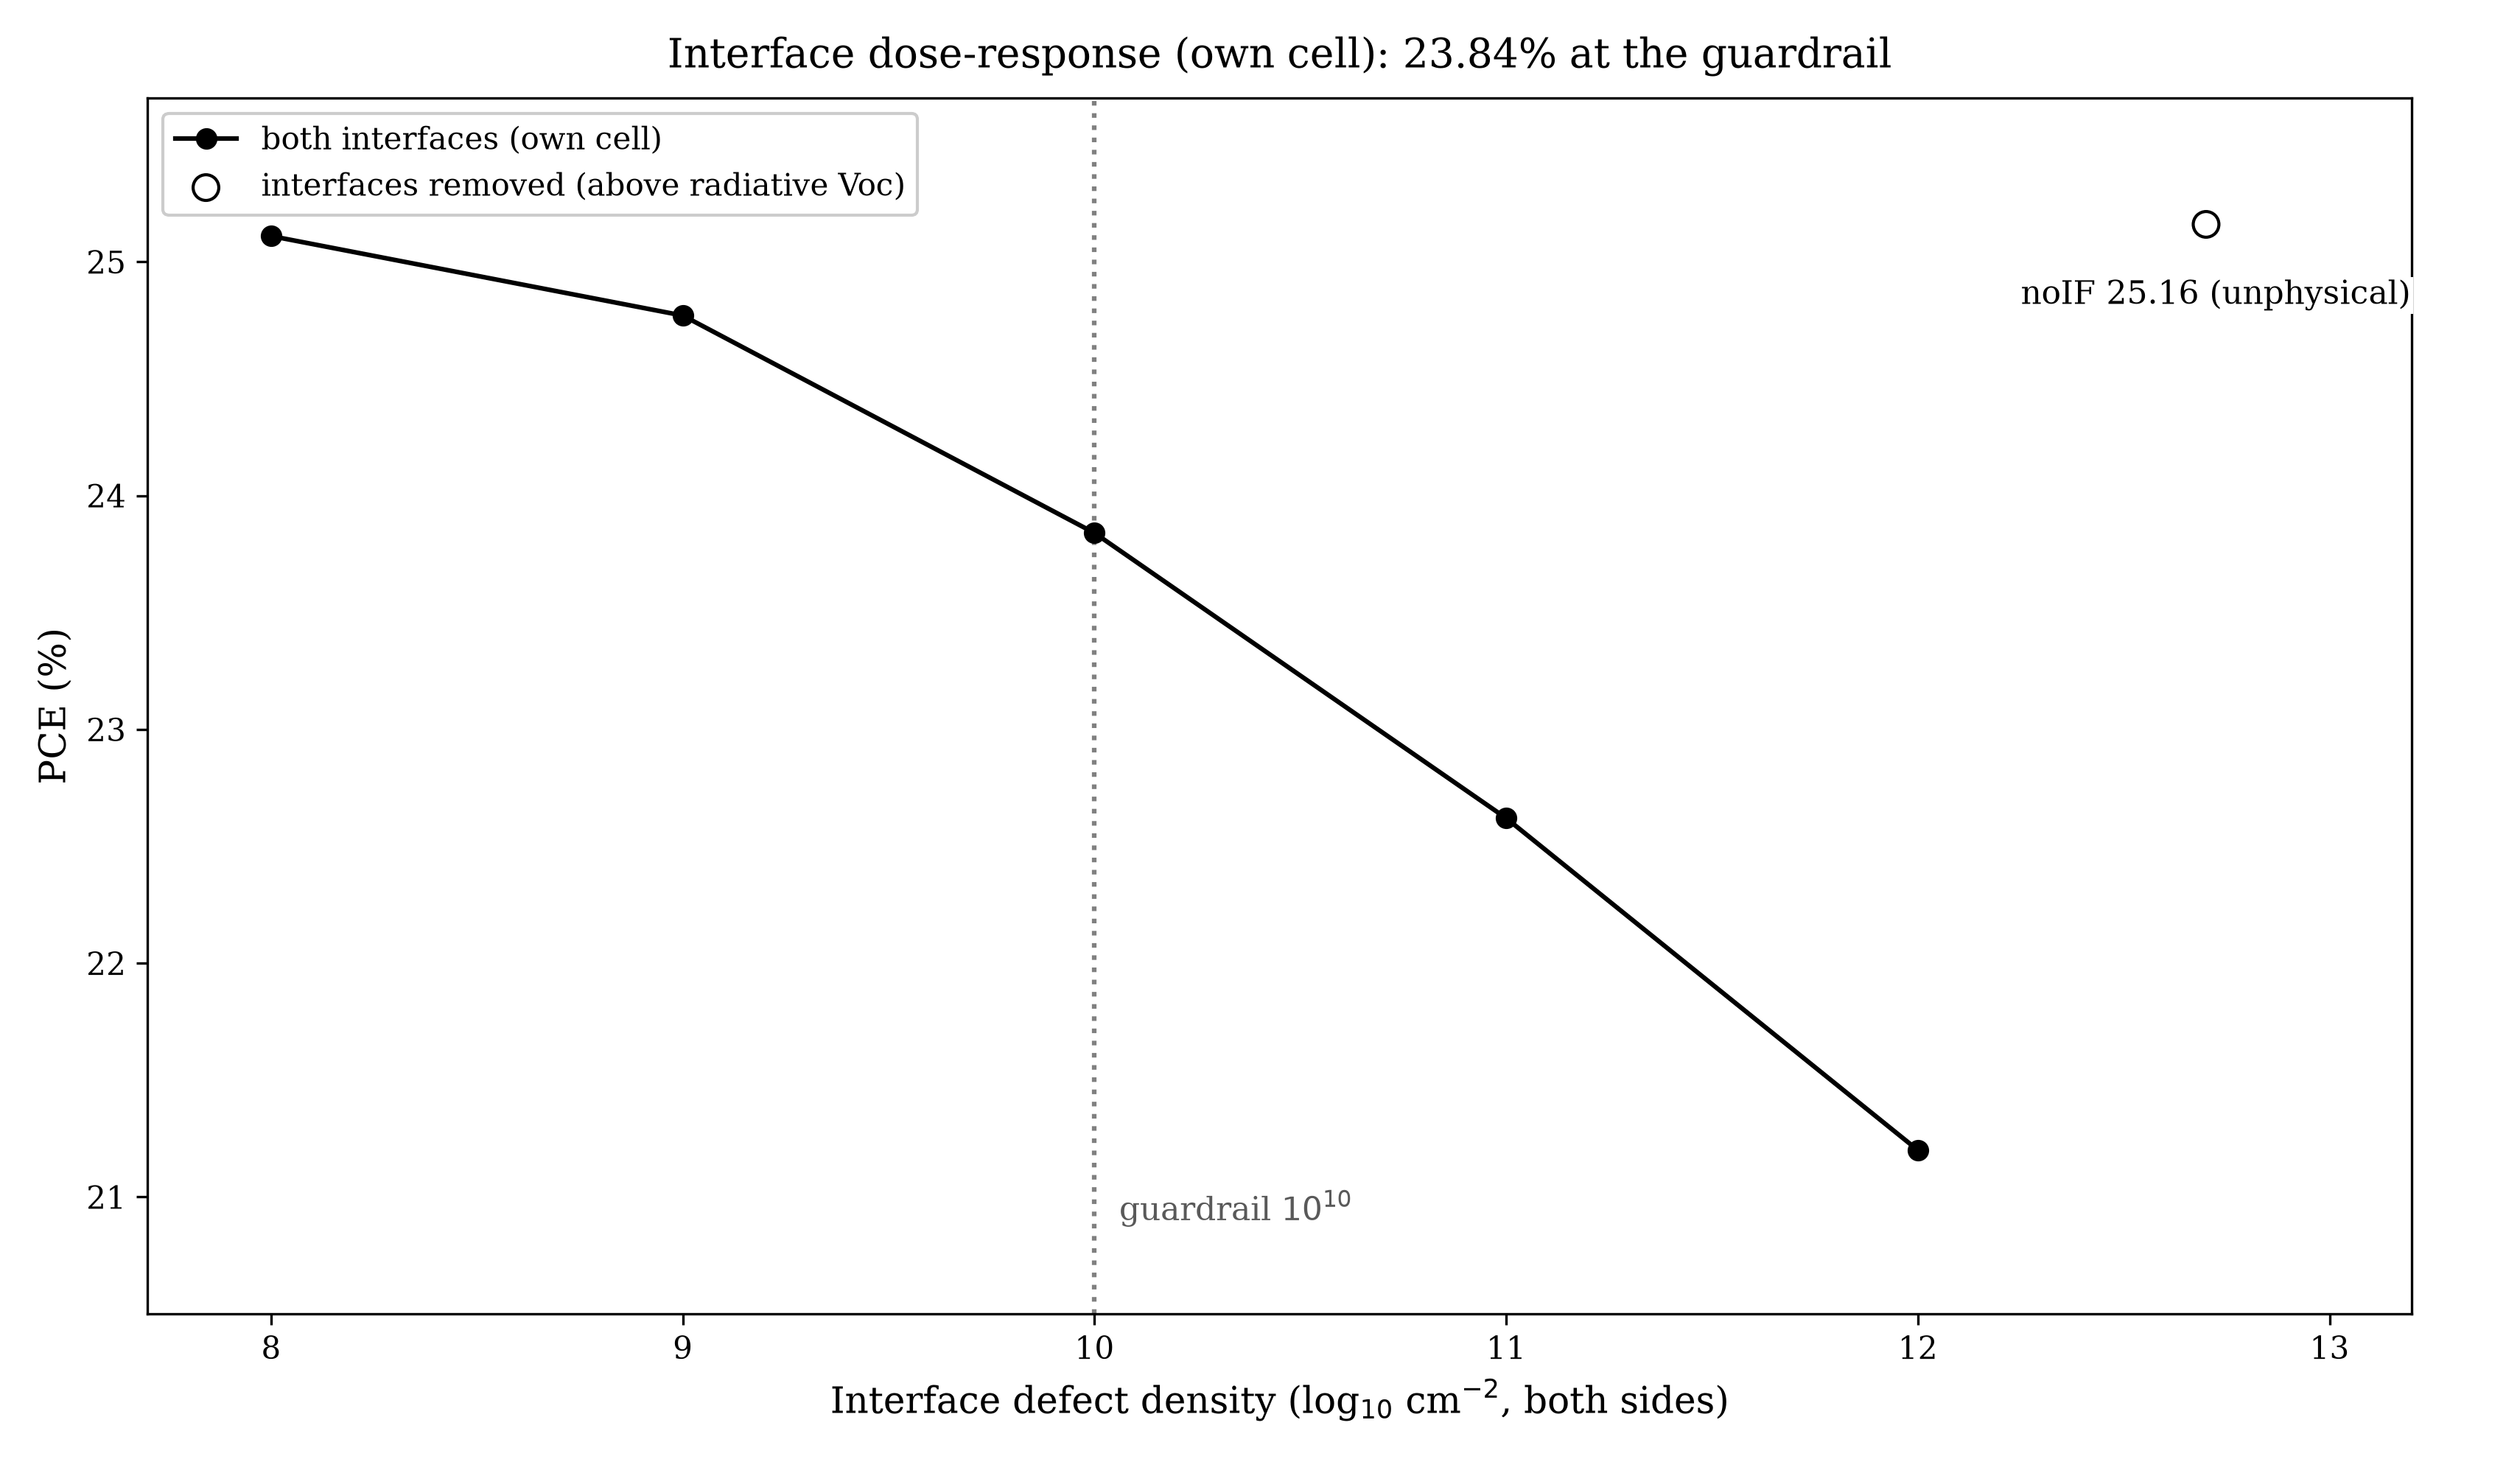
\includegraphics[width=0.8\textwidth]{figs/fig_audit.png}
\caption{Efficiency versus interface density on the prior-adopted base ($\chi_{\mathrm{TiO2}}=3.8$, $E_g=1.65$). The no-interface point (25.16\%) is the surveyed-base audit value from Table~\ref{tab:audit}, shown for scale as an audit point, not a candidate.}
\label{fig:audit}
\end{figure}

\begin{table}[tbp]
\centering
\caption{Guardrailed regime in portable metrics with $\sigma=10^{-19}$~m$^2$ and $v_{th}=10^5$~m/s: bulk lifetime $\tau$ and interface velocity $S$.}
\label{tab:taus}
\begin{tabular}{|l|l|l|}
\hline\hline
Density & $\tau$ / $S$ & Note \\
\hline
$N_t=10^{12}$~cm$^{-3}$ (floor) & $\tau=100$~$\mu$s & beyond-best-film regime \\
$N_t=10^{13}$~cm$^{-3}$ & $\tau=10$~$\mu$s & -- \\
$N_t=10^{14}$~cm$^{-3}$ & $\tau=1$~$\mu$s & -- \\
$N_t=10^{15}$~cm$^{-3}$ (routine) & $\tau=0.1$~$\mu$s & routine case \\
$N_{if}=10^{10}$~cm$^{-2}$ (floor) & $S=100$~cm/s & floor of stated box \\
$N_{if}=10^{11}$~cm$^{-2}$ & $S=1000$~cm/s & -- \\
\hline\hline
\end{tabular}
\end{table}

\begin{table}[tbp]
\centering
\caption{Identical cells with interfaces ON versus OFF.}
\label{tab:audit}
\begin{tabular}{|l|l|l|l|}
\hline\hline
Cell & IF ON (\%) & IF OFF (\%) & Inflation (pts) \\
\hline
1.5~$\mu$m cell & 23.40 & 24.87 & +1.47 \\
2.0~$\mu$m cell & 23.47 & 24.73 & +1.26 \\
Surveyed-base best & 23.50 & 25.16 & +1.66 \\
\hline\hline
\end{tabular}
\end{table}

No-interface Voc values sit at or very near the model-derived radiative bound because the model omits a radiative channel. Those cells are therefore disqualified by lack of margin, not ranked.

\subsection{Morris sensitivity}

A guardrail-clean Morris screen used eight trajectories, four levels, six factors, and 56 converged runs spanning 15.34--22.96\%. Per decade, interfaces lead at 0.85 points against 0.37 for bulk defects, but their bootstrap intervals overlap. The sharper paired-trajectory difference is +0.58 points with interval [-0.59, 1.97], with five of eight trajectories positive. Morris alone therefore does not establish the interface lead.

\begin{figure}[tbp]
\centering
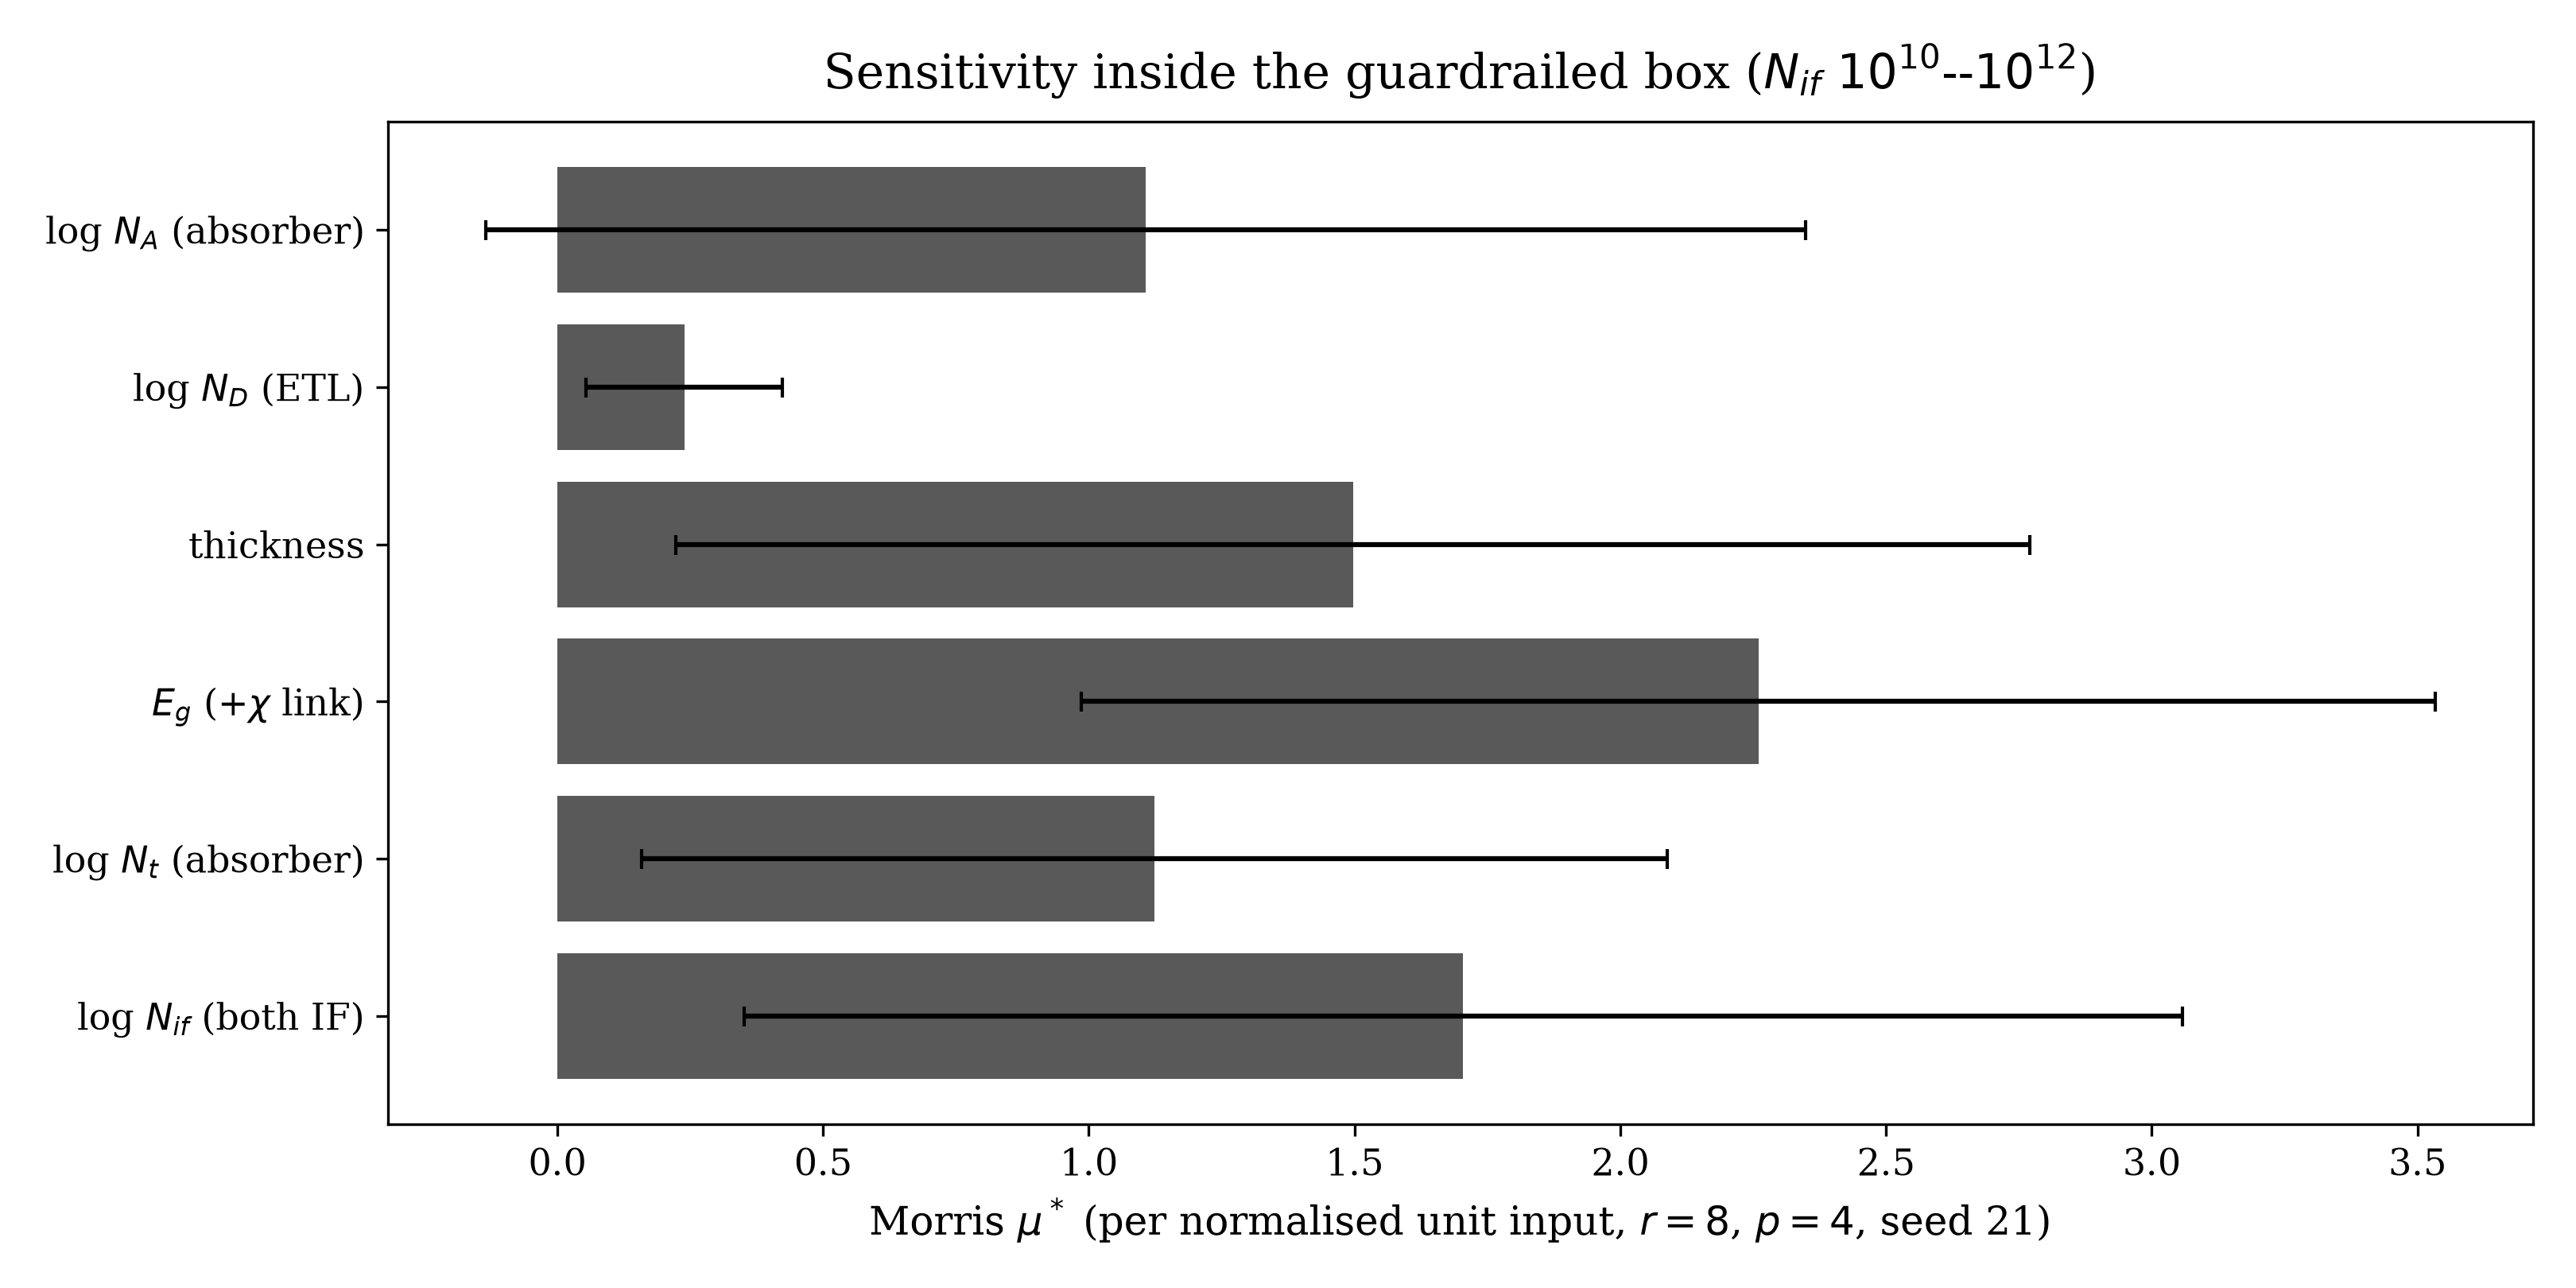
\includegraphics[width=0.8\textwidth]{figs/fig_morris.png}
\caption{Morris $\mu^*$ with interaction spread $\sigma$. Rankings are regime conditional and use different physical units across factors.}
\label{fig:morris}
\end{figure}

The regime conclusion instead rests on the dose--response and the nominal $S$ versus $d/\tau$ anchors~\cite{Sproul1994}. Those anchors organise the clean-corner and routine-defect regimes; binning the prior-volume runs by the same ratio does not reveal a clean internal crossing at this sample size. The same nominal interface velocity can also recombine differently as alignment changes the interface carrier densities.

\subsection{Loss budget and limits}

The ceiling exceeds the certified record by 2.93 points at 1.65~eV (24.95 versus 22.02\%) and by 2.71 points even at 1.70~eV (24.73\%, Voc 1.364~V, Jsc 20.23~mA/cm$^2$, FF 89.58\%; receipts \texttt{outputs/s36\_rs.json}). The excess cannot be assigned to the gap alone. Simulated fill factor near 89\% exceeds measured values near 83\%, alongside permissive contacts and affinities.

\begin{table}[tbp]
\centering
\caption{Loss budget: permissive-box ceiling against measured devices and model limits. The Lei row mixes printed and headline values as stated in its source.}
\label{tab:loss}
\begin{tabular}{|l|l|l|l|l|}
\hline\hline
Device & Voc (V) & Jsc (mA/cm$^2$) & FF (\%) & PCE (\%) \\
\hline
This work (box ceiling) & 1.321 & 21.20 & 89.11 & 24.95 \\
This work + $C_r=10^{-10}$ & 1.163 & 21.08 & 89.13 & 21.86 \\
This work, stacked realistic range & 1.19 & 18.9--19.4 & 83.6--85.5 & 19.25--19.59 \\
AP-modified CsPbI3~\cite{Lei2025} & 1.29 & 20.77 & 83.01 & 22.16 \\
QD-interface CsPbI3~\cite{XuQD2026} & 1.28 & -- & -- & 22.15 \\
Dual-interface CsPbI3~\cite{Zhang2026} & 1.27 & -- & -- & 21.71 \\
Carbon HTL-free~\cite{LiCarbon2026} & 1.202 & 20.72 & 83.2 & 20.72 \\
Model-derived radiative bound, this stack (1.65~eV) & 1.371 & 24.4 step-absorption reference & 90.5 & -- \\
\hline\hline
\end{tabular}
\end{table}

The approximately six-point fill-factor discrepancy (89.11\% simulated versus $\sim$83\% measured) is the largest remaining gap and is now bounded rather than unresolved. Scripted $R_s=3$--5~$\Omega$cm$^2$ lowers ceiling fill factor to 84.50--81.45\% and routine fill factor to 82.32--78.99\% (Table~\ref{tab:rs}), so measured series resistance accounts for roughly half the gap at plausible $R_s$ values. A missing back reflector affects Jsc rather than fill factor, so it is not offered as the explanation. The remainder is attributed to nonradiative interface recombination (ideality above unity); ideality-factor and illumination-dependent data sufficient to separate the two losses exactly are unavailable, so the decomposition is reported as a bound.

This is one stack, one solver, and one dimension. Several contact cliffs are SCAPS boundary behaviour as much as device physics. The checklist above (Table~\ref{tab:checklist}) is therefore a proposed pilot reporting standard, not an established publication standard.

\begin{table}[tbp]
\centering
\caption{Pilot guardrailed-reporting checklist for comparable SCAPS claims. The full protocol mapping is in Supplement S7.}
\label{tab:checklist}
\small
\begingroup
\setlength{\tabcolsep}{3pt}
\begin{tabular}{|p{0.15\linewidth}|p{0.29\linewidth}|p{0.29\linewidth}|p{0.14\linewidth}|}
\hline\hline
Item & Disclose & This work & Protocol \\
\hline
Interfaces & status + $N_{if}$ + $\sigma$ or $S$ & $10^{10}$~cm$^{-2}$, $10^{-19}$~m$^2$ & reporting \\
Bulk defects & $N_t$ + $\sigma$ or $\tau$ & $10^{12}$~cm$^{-3}$; routine $10^{15}$ & reporting \\
Radiative coefficient & $C_r$ value used & $0$, priced at $10^{-10}$/$10^{-9}$ & inputs \\
Mobilities & $\mu_n$/$\mu_p$ plus anchor & 25/25, priced at 10/5, 5/2 & inputs \\
Units and scripts & script versus file systems & Supplement S2 & reporting \\
Parasitics & $R_s$/$R_{sh}$ basis & scripted; routine case included & inputs \\
Contacts and affinities & work functions and surveyed/adopted $\chi$ & priced & inputs \\
Optics and current & reflection, absorption, spectrum, QE/IV treatment & uncertainty carried & spectra \\
Radiative screen & model-derived Voc bound and deviations & 1.371~V at 1.65~eV (in-model; independent step-absorption Jsc 24.4 in \texttt{outputs/s18\_analytic.json}) & radiative check \\
Receipts & definitions plus raw outputs & public repository, Supplement S1 & reporting \\
\hline\hline
\end{tabular}
\endgroup
\end{table}

\section{Summary}

Factorial screening under interface-inclusive guardrails gives a 24.95\% permissive-box ceiling and an 18.0\% routine-quality prior-predictive envelope on the stated CsPbI3/CBTS stack. Every load-bearing assumption is priced: defect floors, gap, contacts, affinities, radiative recombination, mobility, parasitics to $R_s=5$~$\Omega$cm$^2$, optics, and density of states. The 2024--2026 records lie above the routine envelope. The record comparison for the ceiling is density-of-states conditional and is reported both ways. The principal remaining discrepancy is fill factor, bounded as approximately half resistive and half recombination-driven.

\section*{Data availability}

The simulation archive is based on repository revision \texttt{6e991c1}. The revised manuscript and new supplement are text-level additions to that revision; the revision itself does not claim a new immutable archive hash. Definition files carry the base, no-interface, work-function, and cross-section variants. Sweep receipts, raw curves, scripts, verification receipts, and typeset sources are in the public repository at \url{https://github.com/touhidsiddiqueeraj-bit/Modeling-electricModeling-electrical-losses-in-CsPbI3-solar-cells-al-losses-in-CsPbI3-solar-cells-}. Copyrighted reference PDFs are listed, not redistributed.

\section*{Author contributions}

Hussain Touhid Siddiquee: conceptualization, methodology, software, formal analysis, investigation, data curation, visualization, validation, and writing---original draft, review and editing. Md.\ Abdul Malek Fahim: software, validation, and writing---original draft.

\section*{AI-use declaration}

AI assistance was used during this revision for editing, consistency checking, reference-label correction, and figure-label correction. All SCAPS results come from the archived simulation receipts and were not generated by AI.

\section*{Acknowledgements}

The SCAPS-1D program was kindly provided by Prof.~M.~Burgelman of the University of Gent. Simulation time was provided by local workstation hardware.

\bibliographystyle{unsrtnat}
\bibliography{references}

\end{document}
